\documentclass[twoside]{book}

% Packages required by doxygen
\usepackage{calc}
\usepackage{doxygen}
\usepackage{graphicx}
\usepackage[utf8]{inputenc}
\usepackage{makeidx}
\usepackage{multicol}
\usepackage{multirow}
\usepackage{fixltx2e}
\PassOptionsToPackage{warn}{textcomp}
\usepackage{textcomp}
\usepackage[nointegrals]{wasysym}
\usepackage[table]{xcolor}

% Font selection
\usepackage[T1]{fontenc}
\usepackage{mathptmx}
\usepackage[scaled=.90]{helvet}
\usepackage{courier}
\usepackage{amssymb}
\usepackage{sectsty}
\renewcommand{\familydefault}{\sfdefault}
\allsectionsfont{%
  \fontseries{bc}\selectfont%
  \color{darkgray}%
}
\renewcommand{\DoxyLabelFont}{%
  \fontseries{bc}\selectfont%
  \color{darkgray}%
}
\newcommand{\+}{\discretionary{\mbox{\scriptsize$\hookleftarrow$}}{}{}}

% Page & text layout
\usepackage{geometry}
\geometry{%
  a4paper,%
  top=2.5cm,%
  bottom=2.5cm,%
  left=2.5cm,%
  right=2.5cm%
}
\tolerance=750
\hfuzz=15pt
\hbadness=750
\setlength{\emergencystretch}{15pt}
\setlength{\parindent}{0cm}
\setlength{\parskip}{0.2cm}
\makeatletter
\renewcommand{\paragraph}{%
  \@startsection{paragraph}{4}{0ex}{-1.0ex}{1.0ex}{%
    \normalfont\normalsize\bfseries\SS@parafont%
  }%
}
\renewcommand{\subparagraph}{%
  \@startsection{subparagraph}{5}{0ex}{-1.0ex}{1.0ex}{%
    \normalfont\normalsize\bfseries\SS@subparafont%
  }%
}
\makeatother

% Headers & footers
\usepackage{fancyhdr}
\pagestyle{fancyplain}
\fancyhead[LE]{\fancyplain{}{\bfseries\thepage}}
\fancyhead[CE]{\fancyplain{}{}}
\fancyhead[RE]{\fancyplain{}{\bfseries\leftmark}}
\fancyhead[LO]{\fancyplain{}{\bfseries\rightmark}}
\fancyhead[CO]{\fancyplain{}{}}
\fancyhead[RO]{\fancyplain{}{\bfseries\thepage}}
\fancyfoot[LE]{\fancyplain{}{}}
\fancyfoot[CE]{\fancyplain{}{}}
\fancyfoot[RE]{\fancyplain{}{\bfseries\scriptsize Generated on Sun Jun 1 2014 20\+:33\+:44 for My Project by Doxygen }}
\fancyfoot[LO]{\fancyplain{}{\bfseries\scriptsize Generated on Sun Jun 1 2014 20\+:33\+:44 for My Project by Doxygen }}
\fancyfoot[CO]{\fancyplain{}{}}
\fancyfoot[RO]{\fancyplain{}{}}
\renewcommand{\footrulewidth}{0.4pt}
\renewcommand{\chaptermark}[1]{%
  \markboth{#1}{}%
}
\renewcommand{\sectionmark}[1]{%
  \markright{\thesection\ #1}%
}

% Indices & bibliography
\usepackage{natbib}
\usepackage[titles]{tocloft}
\setcounter{tocdepth}{3}
\setcounter{secnumdepth}{5}
\makeindex

% Hyperlinks (required, but should be loaded last)
\usepackage{ifpdf}
\ifpdf
  \usepackage[pdftex,pagebackref=true]{hyperref}
\else
  \usepackage[ps2pdf,pagebackref=true]{hyperref}
\fi
\hypersetup{%
  colorlinks=true,%
  linkcolor=blue,%
  citecolor=blue,%
  unicode%
}

% Custom commands
\newcommand{\clearemptydoublepage}{%
  \newpage{\pagestyle{empty}\cleardoublepage}%
}


%===== C O N T E N T S =====

\begin{document}

% Titlepage & ToC
\hypersetup{pageanchor=false,
             bookmarks=true,
             bookmarksnumbered=true,
             pdfencoding=unicode
            }
\pagenumbering{roman}
\begin{titlepage}
\vspace*{7cm}
\begin{center}%
{\Large My Project }\\
\vspace*{1cm}
{\large Generated by Doxygen 1.8.7}\\
\vspace*{0.5cm}
{\small Sun Jun 1 2014 20:33:44}\\
\end{center}
\end{titlepage}
\clearemptydoublepage
\tableofcontents
\clearemptydoublepage
\pagenumbering{arabic}
\hypersetup{pageanchor=true}

%--- Begin generated contents ---
\chapter{Namespace Index}
\section{Namespace List}
Here is a list of all documented namespaces with brief descriptions\+:\begin{DoxyCompactList}
\item\contentsline{section}{\hyperlink{namespace_empire___simulator}{Empire\+\_\+\+Simulator} }{\pageref{namespace_empire___simulator}}{}
\item\contentsline{section}{\hyperlink{namespace_empire___simulator_1_1_properties}{Empire\+\_\+\+Simulator.\+Properties} }{\pageref{namespace_empire___simulator_1_1_properties}}{}
\item\contentsline{section}{\hyperlink{namespace_empire___simulator_1_1_wyjatki}{Empire\+\_\+\+Simulator.\+Wyjatki} }{\pageref{namespace_empire___simulator_1_1_wyjatki}}{}
\end{DoxyCompactList}

\chapter{Hierarchical Index}
\section{Class Hierarchy}
This inheritance list is sorted roughly, but not completely, alphabetically\+:\begin{DoxyCompactList}
\item \contentsline{section}{Empire\+\_\+\+Simulator.\+Aktualizacja\+Handlarzy}{\pageref{class_empire___simulator_1_1_aktualizacja_handlarzy}}{}
\item \contentsline{section}{Empire\+\_\+\+Simulator.\+Aktualizacja\+Osad}{\pageref{class_empire___simulator_1_1_aktualizacja_osad}}{}
\item \contentsline{section}{Empire\+\_\+\+Simulator.\+Aktualizacja\+Stanu\+Swiata}{\pageref{class_empire___simulator_1_1_aktualizacja_stanu_swiata}}{}
\item \contentsline{section}{Empire\+\_\+\+Simulator.\+Aktualizator\+Mapy}{\pageref{class_empire___simulator_1_1_aktualizator_mapy}}{}
\item Alpha\+Blend\+Text\+Box\begin{DoxyCompactList}
\item \contentsline{section}{Empire\+\_\+\+Simulator.\+Text\+Box\+Label}{\pageref{class_empire___simulator_1_1_text_box_label}}{}
\end{DoxyCompactList}
\item Application\+Exception\begin{DoxyCompactList}
\item \contentsline{section}{Empire\+\_\+\+Simulator.\+Wyjatki.\+Excepotion\+Brak\+Zasobu}{\pageref{class_empire___simulator_1_1_wyjatki_1_1_excepotion_brak_zasobu}}{}
\end{DoxyCompactList}
\item \contentsline{section}{Empire\+\_\+\+Simulator.\+Fabryka\+Handlarzy}{\pageref{class_empire___simulator_1_1_fabryka_handlarzy}}{}
\item \contentsline{section}{Empire\+\_\+\+Simulator.\+Fabryka\+Osad}{\pageref{class_empire___simulator_1_1_fabryka_osad}}{}
\item \contentsline{section}{Empire\+\_\+\+Simulator.\+Fabryka\+Zasobow}{\pageref{class_empire___simulator_1_1_fabryka_zasobow}}{}
\item Form\begin{DoxyCompactList}
\item \contentsline{section}{Empire\+\_\+\+Simulator.\+Okno\+Gry}{\pageref{class_empire___simulator_1_1_okno_gry}}{}
\end{DoxyCompactList}
\item \contentsline{section}{Empire\+\_\+\+Simulator.\+Generator\+Mapy}{\pageref{class_empire___simulator_1_1_generator_mapy}}{}
\item \contentsline{section}{Empire\+\_\+\+Simulator.\+Generator\+Swiata}{\pageref{class_empire___simulator_1_1_generator_swiata}}{}
\item \contentsline{section}{Empire\+\_\+\+Simulator.\+Handlarz}{\pageref{class_empire___simulator_1_1_handlarz}}{}
\item \contentsline{section}{Empire\+\_\+\+Simulator.\+I\+Strategia\+Aktualizacji\+Swiata}{\pageref{interface_empire___simulator_1_1_i_strategia_aktualizacji_swiata}}{}
\begin{DoxyCompactList}
\item \contentsline{section}{Empire\+\_\+\+Simulator.\+Podstawowa\+Strategia\+Aktualizacji\+Swiata}{\pageref{class_empire___simulator_1_1_podstawowa_strategia_aktualizacji_swiata}}{}
\end{DoxyCompactList}
\item \contentsline{section}{Empire\+\_\+\+Simulator.\+I\+Strategia\+Generowania\+Swiata}{\pageref{interface_empire___simulator_1_1_i_strategia_generowania_swiata}}{}
\begin{DoxyCompactList}
\item \contentsline{section}{Empire\+\_\+\+Simulator.\+Podstawowa\+Strategia\+Generowania\+Swiata}{\pageref{class_empire___simulator_1_1_podstawowa_strategia_generowania_swiata}}{}
\end{DoxyCompactList}
\item \contentsline{section}{Empire\+\_\+\+Simulator.\+I\+Strategia\+Handlarza}{\pageref{interface_empire___simulator_1_1_i_strategia_handlarza}}{}
\begin{DoxyCompactList}
\item \contentsline{section}{Empire\+\_\+\+Simulator.\+Podstawowa\+Strategia\+Handlarza}{\pageref{class_empire___simulator_1_1_podstawowa_strategia_handlarza}}{}
\end{DoxyCompactList}
\item \contentsline{section}{Empire\+\_\+\+Simulator.\+I\+Strategia\+Handlu}{\pageref{interface_empire___simulator_1_1_i_strategia_handlu}}{}
\begin{DoxyCompactList}
\item \contentsline{section}{Empire\+\_\+\+Simulator.\+Podstawowa\+Strategia\+Handlu}{\pageref{class_empire___simulator_1_1_podstawowa_strategia_handlu}}{}
\end{DoxyCompactList}
\item \contentsline{section}{Empire\+\_\+\+Simulator.\+I\+Strategia\+Osady}{\pageref{interface_empire___simulator_1_1_i_strategia_osady}}{}
\begin{DoxyCompactList}
\item \contentsline{section}{Empire\+\_\+\+Simulator.\+Podstawowa\+Strategia\+Osady}{\pageref{class_empire___simulator_1_1_podstawowa_strategia_osady}}{}
\end{DoxyCompactList}
\item \contentsline{section}{Empire\+\_\+\+Simulator.\+Losowanie\+Potencjalu}{\pageref{class_empire___simulator_1_1_losowanie_potencjalu}}{}
\item \contentsline{section}{Empire\+\_\+\+Simulator.\+Losowanie\+Zasobu}{\pageref{class_empire___simulator_1_1_losowanie_zasobu}}{}
\item \contentsline{section}{Empire\+\_\+\+Simulator.\+Magazyn}{\pageref{class_empire___simulator_1_1_magazyn}}{}
\item \contentsline{section}{Empire\+\_\+\+Simulator.\+Osada}{\pageref{class_empire___simulator_1_1_osada}}{}
\item \contentsline{section}{Empire\+\_\+\+Simulator.\+Populacja}{\pageref{class_empire___simulator_1_1_populacja}}{}
\item \contentsline{section}{Empire\+\_\+\+Simulator.\+Potencjal\+Wydobywczy}{\pageref{class_empire___simulator_1_1_potencjal_wydobywczy}}{}
\item \contentsline{section}{Empire\+\_\+\+Simulator.\+Swiat}{\pageref{class_empire___simulator_1_1_swiat}}{}
\item \contentsline{section}{Empire\+\_\+\+Simulator.\+Targ}{\pageref{class_empire___simulator_1_1_targ}}{}
\item \contentsline{section}{Empire\+\_\+\+Simulator.\+Test}{\pageref{class_empire___simulator_1_1_test}}{}
\item \contentsline{section}{Empire\+\_\+\+Simulator.\+Woz\+Handlarza}{\pageref{class_empire___simulator_1_1_woz_handlarza}}{}
\item \contentsline{section}{Empire\+\_\+\+Simulator.\+Zasob}{\pageref{class_empire___simulator_1_1_zasob}}{}
\end{DoxyCompactList}

\chapter{Class Index}
\section{Class List}
Here are the classes, structs, unions and interfaces with brief descriptions\+:\begin{DoxyCompactList}
\item\contentsline{section}{\hyperlink{class_empire___simulator_1_1_aktualizacja_handlarzy}{Empire\+\_\+\+Simulator.\+Aktualizacja\+Handlarzy} }{\pageref{class_empire___simulator_1_1_aktualizacja_handlarzy}}{}
\item\contentsline{section}{\hyperlink{class_empire___simulator_1_1_aktualizacja_osad}{Empire\+\_\+\+Simulator.\+Aktualizacja\+Osad} }{\pageref{class_empire___simulator_1_1_aktualizacja_osad}}{}
\item\contentsline{section}{\hyperlink{class_empire___simulator_1_1_aktualizacja_stanu_swiata}{Empire\+\_\+\+Simulator.\+Aktualizacja\+Stanu\+Swiata} \\*Jest to klasa której obiekt jest wstanie zaktualizowac caly stan swiata. }{\pageref{class_empire___simulator_1_1_aktualizacja_stanu_swiata}}{}
\item\contentsline{section}{\hyperlink{class_empire___simulator_1_1_aktualizator_mapy}{Empire\+\_\+\+Simulator.\+Aktualizator\+Mapy} \\*Obiekt aktualizatora mapy sprawdza czy zaszły jakies zmiany w świecie (wielkosc wioski, pozycja handlarza) i koryguje te zmiany na mapie }{\pageref{class_empire___simulator_1_1_aktualizator_mapy}}{}
\item\contentsline{section}{\hyperlink{class_empire___simulator_1_1_wyjatki_1_1_excepotion_brak_zasobu}{Empire\+\_\+\+Simulator.\+Wyjatki.\+Excepotion\+Brak\+Zasobu} }{\pageref{class_empire___simulator_1_1_wyjatki_1_1_excepotion_brak_zasobu}}{}
\item\contentsline{section}{\hyperlink{class_empire___simulator_1_1_fabryka_handlarzy}{Empire\+\_\+\+Simulator.\+Fabryka\+Handlarzy} \\*generuje handlarzy z podana strategią i iloscia towaru ktora mogą ze sobą wozić. }{\pageref{class_empire___simulator_1_1_fabryka_handlarzy}}{}
\item\contentsline{section}{\hyperlink{class_empire___simulator_1_1_fabryka_osad}{Empire\+\_\+\+Simulator.\+Fabryka\+Osad} \\*Klasa która tworzy Osady }{\pageref{class_empire___simulator_1_1_fabryka_osad}}{}
\item\contentsline{section}{\hyperlink{class_empire___simulator_1_1_fabryka_zasobow}{Empire\+\_\+\+Simulator.\+Fabryka\+Zasobow} \\*Fabryka Zasobow to klasa ktora potrafi generowac gotowe do uzycia obiekty zasobow na podstawie swoich danyh }{\pageref{class_empire___simulator_1_1_fabryka_zasobow}}{}
\item\contentsline{section}{\hyperlink{class_empire___simulator_1_1_generator_mapy}{Empire\+\_\+\+Simulator.\+Generator\+Mapy} \\*Obiekt generatora mapy pozwala na naniesienie osad,handlarzy i tła na ramkę gry }{\pageref{class_empire___simulator_1_1_generator_mapy}}{}
\item\contentsline{section}{\hyperlink{class_empire___simulator_1_1_generator_swiata}{Empire\+\_\+\+Simulator.\+Generator\+Swiata} \\*Jest to klasa której obiekt potrafi wygenerowac swiat na podstawie podanej strategi }{\pageref{class_empire___simulator_1_1_generator_swiata}}{}
\item\contentsline{section}{\hyperlink{class_empire___simulator_1_1_handlarz}{Empire\+\_\+\+Simulator.\+Handlarz} }{\pageref{class_empire___simulator_1_1_handlarz}}{}
\item\contentsline{section}{\hyperlink{interface_empire___simulator_1_1_i_strategia_aktualizacji_swiata}{Empire\+\_\+\+Simulator.\+I\+Strategia\+Aktualizacji\+Swiata} \\*Interfejs Aktualizacji swiata ma metody zwracajace to co ile dni handlarz zmienia swój stan, podobnie tyczy się to wioski }{\pageref{interface_empire___simulator_1_1_i_strategia_aktualizacji_swiata}}{}
\item\contentsline{section}{\hyperlink{interface_empire___simulator_1_1_i_strategia_generowania_swiata}{Empire\+\_\+\+Simulator.\+I\+Strategia\+Generowania\+Swiata} \\*Jest to ogolny interfejs generowania swiata, ktory mówi o tym ile osad wygenerowac na mapie, ilu handlarzy,i jaka pojemność bedzie miał wóz handlarze podaje też z jakich strategi handlarza,handlu i Osady bedziemy korzystac }{\pageref{interface_empire___simulator_1_1_i_strategia_generowania_swiata}}{}
\item\contentsline{section}{\hyperlink{interface_empire___simulator_1_1_i_strategia_handlarza}{Empire\+\_\+\+Simulator.\+I\+Strategia\+Handlarza} \\*Interfejs mówiący o tym jak wyznaczać nowy cel podróży dla handlarza oraz w jaki sposob sie przemieszcza }{\pageref{interface_empire___simulator_1_1_i_strategia_handlarza}}{}
\item\contentsline{section}{\hyperlink{interface_empire___simulator_1_1_i_strategia_handlu}{Empire\+\_\+\+Simulator.\+I\+Strategia\+Handlu} \\*interfejs opisujacy jak wyglada wymiana towaru miedzy targiem a handlarzem }{\pageref{interface_empire___simulator_1_1_i_strategia_handlu}}{}
\item\contentsline{section}{\hyperlink{interface_empire___simulator_1_1_i_strategia_osady}{Empire\+\_\+\+Simulator.\+I\+Strategia\+Osady} \\*Interfejs strategi osady wymusza metody których używa osada do zaktualizowania swojego statusu tj. stanow magazynowych i populacji, strategie bedą wymienne }{\pageref{interface_empire___simulator_1_1_i_strategia_osady}}{}
\item\contentsline{section}{\hyperlink{class_empire___simulator_1_1_losowanie_potencjalu}{Empire\+\_\+\+Simulator.\+Losowanie\+Potencjalu} \\*zwraca liste wylosowanych zasobow. }{\pageref{class_empire___simulator_1_1_losowanie_potencjalu}}{}
\item\contentsline{section}{\hyperlink{class_empire___simulator_1_1_losowanie_zasobu}{Empire\+\_\+\+Simulator.\+Losowanie\+Zasobu} \\*Tworzy obiekt potrafiacy wylosowac liczbe z zadanego mu przedzialu }{\pageref{class_empire___simulator_1_1_losowanie_zasobu}}{}
\item\contentsline{section}{\hyperlink{class_empire___simulator_1_1_magazyn}{Empire\+\_\+\+Simulator.\+Magazyn} \\*\hyperlink{class_empire___simulator_1_1_magazyn}{Magazyn} jest obiektem posiadanym przez osadę, i przetrzymującym w swoich polach ilośći zasobów posiadane przez ową wioskę }{\pageref{class_empire___simulator_1_1_magazyn}}{}
\item\contentsline{section}{\hyperlink{class_empire___simulator_1_1_okno_gry}{Empire\+\_\+\+Simulator.\+Okno\+Gry} \\*Jest to główne okno gry }{\pageref{class_empire___simulator_1_1_okno_gry}}{}
\item\contentsline{section}{\hyperlink{class_empire___simulator_1_1_osada}{Empire\+\_\+\+Simulator.\+Osada} \\*Klasa Tworzaca obiekt osady }{\pageref{class_empire___simulator_1_1_osada}}{}
\item\contentsline{section}{\hyperlink{class_empire___simulator_1_1_podstawowa_strategia_aktualizacji_swiata}{Empire\+\_\+\+Simulator.\+Podstawowa\+Strategia\+Aktualizacji\+Swiata} }{\pageref{class_empire___simulator_1_1_podstawowa_strategia_aktualizacji_swiata}}{}
\item\contentsline{section}{\hyperlink{class_empire___simulator_1_1_podstawowa_strategia_generowania_swiata}{Empire\+\_\+\+Simulator.\+Podstawowa\+Strategia\+Generowania\+Swiata} }{\pageref{class_empire___simulator_1_1_podstawowa_strategia_generowania_swiata}}{}
\item\contentsline{section}{\hyperlink{class_empire___simulator_1_1_podstawowa_strategia_handlarza}{Empire\+\_\+\+Simulator.\+Podstawowa\+Strategia\+Handlarza} }{\pageref{class_empire___simulator_1_1_podstawowa_strategia_handlarza}}{}
\item\contentsline{section}{\hyperlink{class_empire___simulator_1_1_podstawowa_strategia_handlu}{Empire\+\_\+\+Simulator.\+Podstawowa\+Strategia\+Handlu} }{\pageref{class_empire___simulator_1_1_podstawowa_strategia_handlu}}{}
\item\contentsline{section}{\hyperlink{class_empire___simulator_1_1_podstawowa_strategia_osady}{Empire\+\_\+\+Simulator.\+Podstawowa\+Strategia\+Osady} \\*Własna strategia implementujaca interfejs strategi osady }{\pageref{class_empire___simulator_1_1_podstawowa_strategia_osady}}{}
\item\contentsline{section}{\hyperlink{class_empire___simulator_1_1_populacja}{Empire\+\_\+\+Simulator.\+Populacja} \\*Klasa Tworzaca obiekty populacji tj zawierajace informacie o liczbie ludnosci }{\pageref{class_empire___simulator_1_1_populacja}}{}
\item\contentsline{section}{\hyperlink{class_empire___simulator_1_1_potencjal_wydobywczy}{Empire\+\_\+\+Simulator.\+Potencjal\+Wydobywczy} \\*Potencjal wydobywczy bedzie gotowym obiektem zawieajacym liste obiektow zasobu jakie generuje dana osada }{\pageref{class_empire___simulator_1_1_potencjal_wydobywczy}}{}
\item\contentsline{section}{\hyperlink{class_empire___simulator_1_1_swiat}{Empire\+\_\+\+Simulator.\+Swiat} \\*Obekt klasy swiat jest takim \char`\"{}kontenerem\char`\"{} trzymajcaym liste osad i liste handlarzy dostepnych w aktualnym świecie }{\pageref{class_empire___simulator_1_1_swiat}}{}
\item\contentsline{section}{\hyperlink{class_empire___simulator_1_1_targ}{Empire\+\_\+\+Simulator.\+Targ} \\*\hyperlink{class_empire___simulator_1_1_targ}{Targ} posiadany przez miasto i uzywany do komunikacji miedzy handlarzami a miastem }{\pageref{class_empire___simulator_1_1_targ}}{}
\item\contentsline{section}{\hyperlink{class_empire___simulator_1_1_test}{Empire\+\_\+\+Simulator.\+Test} }{\pageref{class_empire___simulator_1_1_test}}{}
\item\contentsline{section}{\hyperlink{class_empire___simulator_1_1_text_box_label}{Empire\+\_\+\+Simulator.\+Text\+Box\+Label} \\*Kod skopiowany z iternetu obsługujący przeźroczystość text\+Boxów }{\pageref{class_empire___simulator_1_1_text_box_label}}{}
\item\contentsline{section}{\hyperlink{class_empire___simulator_1_1_woz_handlarza}{Empire\+\_\+\+Simulator.\+Woz\+Handlarza} \\*klasa woz handlarza bedzie obiektem trzymajacym zasoby przewozone przez Handlarza uzywam slownika dlatego ze w przyszlosci planuje to ze handlarz bedzie wozil kilka roznych towarow }{\pageref{class_empire___simulator_1_1_woz_handlarza}}{}
\item\contentsline{section}{\hyperlink{class_empire___simulator_1_1_zasob}{Empire\+\_\+\+Simulator.\+Zasob} \\*Obiekt zasobu przechowujacy jego nazwe wage i ilosc }{\pageref{class_empire___simulator_1_1_zasob}}{}
\end{DoxyCompactList}

\chapter{Namespace Documentation}
\hypertarget{namespace_empire___simulator}{\section{Package Empire\+\_\+\+Simulator}
\label{namespace_empire___simulator}\index{Empire\+\_\+\+Simulator@{Empire\+\_\+\+Simulator}}
}
\subsection*{Namespaces}
\begin{DoxyCompactItemize}
\item 
package \hyperlink{namespace_empire___simulator_1_1_properties}{Properties}
\item 
package \hyperlink{namespace_empire___simulator_1_1_wyjatki}{Wyjatki}
\end{DoxyCompactItemize}
\subsection*{Classes}
\begin{DoxyCompactItemize}
\item 
class \hyperlink{class_empire___simulator_1_1_aktualizacja_handlarzy}{Aktualizacja\+Handlarzy}
\item 
class \hyperlink{class_empire___simulator_1_1_aktualizacja_osad}{Aktualizacja\+Osad}
\item 
class \hyperlink{class_empire___simulator_1_1_aktualizacja_stanu_swiata}{Aktualizacja\+Stanu\+Swiata}
\begin{DoxyCompactList}\small\item\em Jest to klasa której obiekt jest wstanie zaktualizowac caly stan swiata. \end{DoxyCompactList}\item 
class \hyperlink{class_empire___simulator_1_1_aktualizator_mapy}{Aktualizator\+Mapy}
\begin{DoxyCompactList}\small\item\em Obiekt aktualizatora mapy sprawdza czy zaszły jakies zmiany w świecie (wielkosc wioski, pozycja handlarza) i koryguje te zmiany na mapie \end{DoxyCompactList}\item 
class \hyperlink{class_empire___simulator_1_1_fabryka_handlarzy}{Fabryka\+Handlarzy}
\begin{DoxyCompactList}\small\item\em generuje handlarzy z podana strategią i iloscia towaru ktora mogą ze sobą wozić. \end{DoxyCompactList}\item 
class \hyperlink{class_empire___simulator_1_1_fabryka_osad}{Fabryka\+Osad}
\begin{DoxyCompactList}\small\item\em Klasa która tworzy Osady \end{DoxyCompactList}\item 
class \hyperlink{class_empire___simulator_1_1_fabryka_zasobow}{Fabryka\+Zasobow}
\begin{DoxyCompactList}\small\item\em Fabryka Zasobow to klasa ktora potrafi generowac gotowe do uzycia obiekty zasobow na podstawie swoich danyh \end{DoxyCompactList}\item 
class \hyperlink{class_empire___simulator_1_1_generator_mapy}{Generator\+Mapy}
\begin{DoxyCompactList}\small\item\em Obiekt generatora mapy pozwala na naniesienie osad,handlarzy i tła na ramkę gry \end{DoxyCompactList}\item 
class \hyperlink{class_empire___simulator_1_1_generator_swiata}{Generator\+Swiata}
\begin{DoxyCompactList}\small\item\em Jest to klasa której obiekt potrafi wygenerowac swiat na podstawie podanej strategi \end{DoxyCompactList}\item 
class \hyperlink{class_empire___simulator_1_1_handlarz}{Handlarz}
\item 
interface \hyperlink{interface_empire___simulator_1_1_i_strategia_aktualizacji_swiata}{I\+Strategia\+Aktualizacji\+Swiata}
\begin{DoxyCompactList}\small\item\em Interfejs Aktualizacji swiata ma metody zwracajace to co ile dni handlarz zmienia swój stan, podobnie tyczy się to wioski \end{DoxyCompactList}\item 
interface \hyperlink{interface_empire___simulator_1_1_i_strategia_generowania_swiata}{I\+Strategia\+Generowania\+Swiata}
\begin{DoxyCompactList}\small\item\em Jest to ogolny interfejs generowania swiata, ktory mówi o tym ile osad wygenerowac na mapie, ilu handlarzy,i jaka pojemność bedzie miał wóz handlarze podaje też z jakich strategi handlarza,handlu i Osady bedziemy korzystac \end{DoxyCompactList}\item 
interface \hyperlink{interface_empire___simulator_1_1_i_strategia_handlarza}{I\+Strategia\+Handlarza}
\begin{DoxyCompactList}\small\item\em Interfejs mówiący o tym jak wyznaczać nowy cel podróży dla handlarza oraz w jaki sposob sie przemieszcza \end{DoxyCompactList}\item 
interface \hyperlink{interface_empire___simulator_1_1_i_strategia_handlu}{I\+Strategia\+Handlu}
\begin{DoxyCompactList}\small\item\em interfejs opisujacy jak wyglada wymiana towaru miedzy targiem a handlarzem \end{DoxyCompactList}\item 
interface \hyperlink{interface_empire___simulator_1_1_i_strategia_osady}{I\+Strategia\+Osady}
\begin{DoxyCompactList}\small\item\em Interfejs strategi osady wymusza metody których używa osada do zaktualizowania swojego statusu tj. stanow magazynowych i populacji, strategie bedą wymienne \end{DoxyCompactList}\item 
class \hyperlink{class_empire___simulator_1_1_losowanie_potencjalu}{Losowanie\+Potencjalu}
\begin{DoxyCompactList}\small\item\em zwraca liste wylosowanych zasobow. \end{DoxyCompactList}\item 
class \hyperlink{class_empire___simulator_1_1_losowanie_zasobu}{Losowanie\+Zasobu}
\begin{DoxyCompactList}\small\item\em Tworzy obiekt potrafiacy wylosowac liczbe z zadanego mu przedzialu \end{DoxyCompactList}\item 
class \hyperlink{class_empire___simulator_1_1_magazyn}{Magazyn}
\begin{DoxyCompactList}\small\item\em \hyperlink{class_empire___simulator_1_1_magazyn}{Magazyn} jest obiektem posiadanym przez osadę, i przetrzymującym w swoich polach ilośći zasobów posiadane przez ową wioskę \end{DoxyCompactList}\item 
class \hyperlink{class_empire___simulator_1_1_okno_gry}{Okno\+Gry}
\begin{DoxyCompactList}\small\item\em Jest to główne okno gry \end{DoxyCompactList}\item 
class \hyperlink{class_empire___simulator_1_1_osada}{Osada}
\begin{DoxyCompactList}\small\item\em Klasa Tworzaca obiekt osady \end{DoxyCompactList}\item 
class \hyperlink{class_empire___simulator_1_1_podstawowa_strategia_aktualizacji_swiata}{Podstawowa\+Strategia\+Aktualizacji\+Swiata}
\item 
class \hyperlink{class_empire___simulator_1_1_podstawowa_strategia_generowania_swiata}{Podstawowa\+Strategia\+Generowania\+Swiata}
\item 
class \hyperlink{class_empire___simulator_1_1_podstawowa_strategia_handlarza}{Podstawowa\+Strategia\+Handlarza}
\item 
class \hyperlink{class_empire___simulator_1_1_podstawowa_strategia_handlu}{Podstawowa\+Strategia\+Handlu}
\item 
class \hyperlink{class_empire___simulator_1_1_podstawowa_strategia_osady}{Podstawowa\+Strategia\+Osady}
\begin{DoxyCompactList}\small\item\em Własna strategia implementujaca interfejs strategi osady \end{DoxyCompactList}\item 
class \hyperlink{class_empire___simulator_1_1_populacja}{Populacja}
\begin{DoxyCompactList}\small\item\em Klasa Tworzaca obiekty populacji tj zawierajace informacie o liczbie ludnosci \end{DoxyCompactList}\item 
class \hyperlink{class_empire___simulator_1_1_potencjal_wydobywczy}{Potencjal\+Wydobywczy}
\begin{DoxyCompactList}\small\item\em Potencjal wydobywczy bedzie gotowym obiektem zawieajacym liste obiektow zasobu jakie generuje dana osada \end{DoxyCompactList}\item 
class \hyperlink{class_empire___simulator_1_1_swiat}{Swiat}
\begin{DoxyCompactList}\small\item\em Obekt klasy swiat jest takim \char`\"{}kontenerem\char`\"{} trzymajcaym liste osad i liste handlarzy dostepnych w aktualnym świecie \end{DoxyCompactList}\item 
class \hyperlink{class_empire___simulator_1_1_targ}{Targ}
\begin{DoxyCompactList}\small\item\em \hyperlink{class_empire___simulator_1_1_targ}{Targ} posiadany przez miasto i uzywany do komunikacji miedzy handlarzami a miastem \end{DoxyCompactList}\item 
class \hyperlink{class_empire___simulator_1_1_test}{Test}
\item 
class \hyperlink{class_empire___simulator_1_1_text_box_label}{Text\+Box\+Label}
\begin{DoxyCompactList}\small\item\em Kod skopiowany z iternetu obsługujący przeźroczystość text\+Boxów \end{DoxyCompactList}\item 
class \hyperlink{class_empire___simulator_1_1_woz_handlarza}{Woz\+Handlarza}
\begin{DoxyCompactList}\small\item\em klasa woz handlarza bedzie obiektem trzymajacym zasoby przewozone przez Handlarza uzywam slownika dlatego ze w przyszlosci planuje to ze handlarz bedzie wozil kilka roznych towarow \end{DoxyCompactList}\item 
class \hyperlink{class_empire___simulator_1_1_zasob}{Zasob}
\begin{DoxyCompactList}\small\item\em Obiekt zasobu przechowujacy jego nazwe wage i ilosc \end{DoxyCompactList}\end{DoxyCompactItemize}
\subsection*{Functions}
\begin{DoxyCompactItemize}
\item 
delegate void \hyperlink{namespace_empire___simulator_acf092e88f238b8c325a166a8a76e34d6}{Delegat\+Aktualizacji\+Handlarzy} ()
\begin{DoxyCompactList}\small\item\em klasa Towrzaca obiekt delegata który zawiera w sobie wywoałanie w kolejnosci aktualizacji każdego z handlarzy \end{DoxyCompactList}\item 
delegate void \hyperlink{namespace_empire___simulator_a5dff9041bde3e9a806615f75bce12d3f}{Delegat\+Aktualizacji\+Osad} ()
\begin{DoxyCompactList}\small\item\em klasa towrzaca obiekt delegata który zawiera w sobie wywoałanie w kolejnosci aktualizacji każdej z osad \end{DoxyCompactList}\end{DoxyCompactItemize}


\subsection{Function Documentation}
\hypertarget{namespace_empire___simulator_acf092e88f238b8c325a166a8a76e34d6}{\index{Empire\+\_\+\+Simulator@{Empire\+\_\+\+Simulator}!Delegat\+Aktualizacji\+Handlarzy@{Delegat\+Aktualizacji\+Handlarzy}}
\index{Delegat\+Aktualizacji\+Handlarzy@{Delegat\+Aktualizacji\+Handlarzy}!Empire\+\_\+\+Simulator@{Empire\+\_\+\+Simulator}}
\subsubsection[{Delegat\+Aktualizacji\+Handlarzy}]{\setlength{\rightskip}{0pt plus 5cm}delegate void Empire\+\_\+\+Simulator.\+Delegat\+Aktualizacji\+Handlarzy (
\begin{DoxyParamCaption}
{}
\end{DoxyParamCaption}
)}}\label{namespace_empire___simulator_acf092e88f238b8c325a166a8a76e34d6}


klasa Towrzaca obiekt delegata który zawiera w sobie wywoałanie w kolejnosci aktualizacji każdego z handlarzy 

\hypertarget{namespace_empire___simulator_a5dff9041bde3e9a806615f75bce12d3f}{\index{Empire\+\_\+\+Simulator@{Empire\+\_\+\+Simulator}!Delegat\+Aktualizacji\+Osad@{Delegat\+Aktualizacji\+Osad}}
\index{Delegat\+Aktualizacji\+Osad@{Delegat\+Aktualizacji\+Osad}!Empire\+\_\+\+Simulator@{Empire\+\_\+\+Simulator}}
\subsubsection[{Delegat\+Aktualizacji\+Osad}]{\setlength{\rightskip}{0pt plus 5cm}delegate void Empire\+\_\+\+Simulator.\+Delegat\+Aktualizacji\+Osad (
\begin{DoxyParamCaption}
{}
\end{DoxyParamCaption}
)}}\label{namespace_empire___simulator_a5dff9041bde3e9a806615f75bce12d3f}


klasa towrzaca obiekt delegata który zawiera w sobie wywoałanie w kolejnosci aktualizacji każdej z osad 


\hypertarget{namespace_empire___simulator_1_1_properties}{\section{Package Empire\+\_\+\+Simulator.\+Properties}
\label{namespace_empire___simulator_1_1_properties}\index{Empire\+\_\+\+Simulator.\+Properties@{Empire\+\_\+\+Simulator.\+Properties}}
}
\subsection*{Classes}
\begin{DoxyCompactItemize}
\item 
class {\bfseries Resources}
\begin{DoxyCompactList}\small\item\em Klasa zasobu wymagająca zdefiniowania typu do wyszukiwania zlokalizowanych ciągów itd. \end{DoxyCompactList}\end{DoxyCompactItemize}

\hypertarget{namespace_empire___simulator_1_1_wyjatki}{\section{Package Empire\+\_\+\+Simulator.\+Wyjatki}
\label{namespace_empire___simulator_1_1_wyjatki}\index{Empire\+\_\+\+Simulator.\+Wyjatki@{Empire\+\_\+\+Simulator.\+Wyjatki}}
}
\subsection*{Classes}
\begin{DoxyCompactItemize}
\item 
class \hyperlink{class_empire___simulator_1_1_wyjatki_1_1_excepotion_brak_zasobu}{Excepotion\+Brak\+Zasobu}
\end{DoxyCompactItemize}

\chapter{Class Documentation}
\hypertarget{class_empire___simulator_1_1_aktualizacja_handlarzy}{\section{Empire\+\_\+\+Simulator.\+Aktualizacja\+Handlarzy Class Reference}
\label{class_empire___simulator_1_1_aktualizacja_handlarzy}\index{Empire\+\_\+\+Simulator.\+Aktualizacja\+Handlarzy@{Empire\+\_\+\+Simulator.\+Aktualizacja\+Handlarzy}}
}
\subsection*{Public Member Functions}
\begin{DoxyCompactItemize}
\item 
\hyperlink{class_empire___simulator_1_1_aktualizacja_handlarzy_a4d49f1c7960f74b1b253ee1ac546fd55}{Aktualizacja\+Handlarzy} (List$<$ \hyperlink{class_empire___simulator_1_1_handlarz}{Handlarz} $>$ lista\+Handlarzy)
\begin{DoxyCompactList}\small\item\em metoda pobiera listę handlarzy i uzupelnia delegat o metody aktualizacji kazdego z nich \end{DoxyCompactList}\item 
\hyperlink{namespace_empire___simulator_acf092e88f238b8c325a166a8a76e34d6}{Delegat\+Aktualizacji\+Handlarzy} \hyperlink{class_empire___simulator_1_1_aktualizacja_handlarzy_a0426389d093dbfdfd16735036205dc42}{pobierz\+Gotowy\+Delegat} ()
\begin{DoxyCompactList}\small\item\em zwraca gotowego do użycia delegtata \end{DoxyCompactList}\end{DoxyCompactItemize}


\subsection{Constructor \& Destructor Documentation}
\hypertarget{class_empire___simulator_1_1_aktualizacja_handlarzy_a4d49f1c7960f74b1b253ee1ac546fd55}{\index{Empire\+\_\+\+Simulator\+::\+Aktualizacja\+Handlarzy@{Empire\+\_\+\+Simulator\+::\+Aktualizacja\+Handlarzy}!Aktualizacja\+Handlarzy@{Aktualizacja\+Handlarzy}}
\index{Aktualizacja\+Handlarzy@{Aktualizacja\+Handlarzy}!Empire\+\_\+\+Simulator\+::\+Aktualizacja\+Handlarzy@{Empire\+\_\+\+Simulator\+::\+Aktualizacja\+Handlarzy}}
\subsubsection[{Aktualizacja\+Handlarzy}]{\setlength{\rightskip}{0pt plus 5cm}Empire\+\_\+\+Simulator.\+Aktualizacja\+Handlarzy.\+Aktualizacja\+Handlarzy (
\begin{DoxyParamCaption}
\item[{List$<$ {\bf Handlarz} $>$}]{lista\+Handlarzy}
\end{DoxyParamCaption}
)\hspace{0.3cm}{\ttfamily [inline]}}}\label{class_empire___simulator_1_1_aktualizacja_handlarzy_a4d49f1c7960f74b1b253ee1ac546fd55}


metoda pobiera listę handlarzy i uzupelnia delegat o metody aktualizacji kazdego z nich 


\begin{DoxyParams}{Parameters}
{\em lista\+Handlarzy} & \\
\hline
\end{DoxyParams}


\subsection{Member Function Documentation}
\hypertarget{class_empire___simulator_1_1_aktualizacja_handlarzy_a0426389d093dbfdfd16735036205dc42}{\index{Empire\+\_\+\+Simulator\+::\+Aktualizacja\+Handlarzy@{Empire\+\_\+\+Simulator\+::\+Aktualizacja\+Handlarzy}!pobierz\+Gotowy\+Delegat@{pobierz\+Gotowy\+Delegat}}
\index{pobierz\+Gotowy\+Delegat@{pobierz\+Gotowy\+Delegat}!Empire\+\_\+\+Simulator\+::\+Aktualizacja\+Handlarzy@{Empire\+\_\+\+Simulator\+::\+Aktualizacja\+Handlarzy}}
\subsubsection[{pobierz\+Gotowy\+Delegat}]{\setlength{\rightskip}{0pt plus 5cm}{\bf Delegat\+Aktualizacji\+Handlarzy} Empire\+\_\+\+Simulator.\+Aktualizacja\+Handlarzy.\+pobierz\+Gotowy\+Delegat (
\begin{DoxyParamCaption}
{}
\end{DoxyParamCaption}
)\hspace{0.3cm}{\ttfamily [inline]}}}\label{class_empire___simulator_1_1_aktualizacja_handlarzy_a0426389d093dbfdfd16735036205dc42}


zwraca gotowego do użycia delegtata 

\begin{DoxyReturn}{Returns}

\end{DoxyReturn}


The documentation for this class was generated from the following file\+:\begin{DoxyCompactItemize}
\item 
C\+:/\+Users/\+Paweł/\+Documents/\+Git\+Hub/\+Empire\+\_\+\+Simulator\+\_\+\+V\+S\+\_\+2008/\+Empire\+\_\+\+Simulator/\+Empire\+\_\+\+Simulator/\+Klasy/\+Aktualizacja/\+Delegaty/Aktualizacja\+Handlarzy.\+cs\end{DoxyCompactItemize}

\hypertarget{class_empire___simulator_1_1_aktualizacja_osad}{\section{Empire\+\_\+\+Simulator.\+Aktualizacja\+Osad Class Reference}
\label{class_empire___simulator_1_1_aktualizacja_osad}\index{Empire\+\_\+\+Simulator.\+Aktualizacja\+Osad@{Empire\+\_\+\+Simulator.\+Aktualizacja\+Osad}}
}
\subsection*{Public Member Functions}
\begin{DoxyCompactItemize}
\item 
\hyperlink{class_empire___simulator_1_1_aktualizacja_osad_a6e5a4b007581db9d1046a2dd262cd184}{Aktualizacja\+Osad} (List$<$ \hyperlink{class_empire___simulator_1_1_osada}{Osada} $>$ lista\+Osad)
\begin{DoxyCompactList}\small\item\em metoda pobiera liste osad i dodaje wywołanie metody aktualizuj kazdej z nich do delegata \end{DoxyCompactList}\item 
\hyperlink{namespace_empire___simulator_a5dff9041bde3e9a806615f75bce12d3f}{Delegat\+Aktualizacji\+Osad} \hyperlink{class_empire___simulator_1_1_aktualizacja_osad_a1e46988d87f241a8817595bc20923af8}{pobierz\+Gotowy\+Delegat} ()
\begin{DoxyCompactList}\small\item\em zwraca gotowego delegata \end{DoxyCompactList}\end{DoxyCompactItemize}


\subsection{Constructor \& Destructor Documentation}
\hypertarget{class_empire___simulator_1_1_aktualizacja_osad_a6e5a4b007581db9d1046a2dd262cd184}{\index{Empire\+\_\+\+Simulator\+::\+Aktualizacja\+Osad@{Empire\+\_\+\+Simulator\+::\+Aktualizacja\+Osad}!Aktualizacja\+Osad@{Aktualizacja\+Osad}}
\index{Aktualizacja\+Osad@{Aktualizacja\+Osad}!Empire\+\_\+\+Simulator\+::\+Aktualizacja\+Osad@{Empire\+\_\+\+Simulator\+::\+Aktualizacja\+Osad}}
\subsubsection[{Aktualizacja\+Osad}]{\setlength{\rightskip}{0pt plus 5cm}Empire\+\_\+\+Simulator.\+Aktualizacja\+Osad.\+Aktualizacja\+Osad (
\begin{DoxyParamCaption}
\item[{List$<$ {\bf Osada} $>$}]{lista\+Osad}
\end{DoxyParamCaption}
)\hspace{0.3cm}{\ttfamily [inline]}}}\label{class_empire___simulator_1_1_aktualizacja_osad_a6e5a4b007581db9d1046a2dd262cd184}


metoda pobiera liste osad i dodaje wywołanie metody aktualizuj kazdej z nich do delegata 


\begin{DoxyParams}{Parameters}
{\em lista\+Osad} & \\
\hline
\end{DoxyParams}


\subsection{Member Function Documentation}
\hypertarget{class_empire___simulator_1_1_aktualizacja_osad_a1e46988d87f241a8817595bc20923af8}{\index{Empire\+\_\+\+Simulator\+::\+Aktualizacja\+Osad@{Empire\+\_\+\+Simulator\+::\+Aktualizacja\+Osad}!pobierz\+Gotowy\+Delegat@{pobierz\+Gotowy\+Delegat}}
\index{pobierz\+Gotowy\+Delegat@{pobierz\+Gotowy\+Delegat}!Empire\+\_\+\+Simulator\+::\+Aktualizacja\+Osad@{Empire\+\_\+\+Simulator\+::\+Aktualizacja\+Osad}}
\subsubsection[{pobierz\+Gotowy\+Delegat}]{\setlength{\rightskip}{0pt plus 5cm}{\bf Delegat\+Aktualizacji\+Osad} Empire\+\_\+\+Simulator.\+Aktualizacja\+Osad.\+pobierz\+Gotowy\+Delegat (
\begin{DoxyParamCaption}
{}
\end{DoxyParamCaption}
)\hspace{0.3cm}{\ttfamily [inline]}}}\label{class_empire___simulator_1_1_aktualizacja_osad_a1e46988d87f241a8817595bc20923af8}


zwraca gotowego delegata 

\begin{DoxyReturn}{Returns}

\end{DoxyReturn}


The documentation for this class was generated from the following file\+:\begin{DoxyCompactItemize}
\item 
C\+:/\+Users/\+Paweł/\+Documents/\+Git\+Hub/\+Empire\+\_\+\+Simulator\+\_\+\+V\+S\+\_\+2008/\+Empire\+\_\+\+Simulator/\+Empire\+\_\+\+Simulator/\+Klasy/\+Aktualizacja/\+Delegaty/Aktualizacja\+Osad.\+cs\end{DoxyCompactItemize}

\hypertarget{class_empire___simulator_1_1_aktualizacja_stanu_swiata}{\section{Empire\+\_\+\+Simulator.\+Aktualizacja\+Stanu\+Swiata Class Reference}
\label{class_empire___simulator_1_1_aktualizacja_stanu_swiata}\index{Empire\+\_\+\+Simulator.\+Aktualizacja\+Stanu\+Swiata@{Empire\+\_\+\+Simulator.\+Aktualizacja\+Stanu\+Swiata}}
}


Jest to klasa której obiekt jest wstanie zaktualizowac caly stan swiata.  


\subsection*{Public Member Functions}
\begin{DoxyCompactItemize}
\item 
\hyperlink{class_empire___simulator_1_1_aktualizacja_stanu_swiata_a1bf42c8cb38ac168165548047c84d282}{Aktualizacja\+Stanu\+Swiata} (\hyperlink{class_empire___simulator_1_1_swiat}{Swiat} swiat)
\begin{DoxyCompactList}\small\item\em klasa Aktualizacji\+Stanu\+Swiata przyjmuje w konstruktorze obiekt świata i na jego podstawie tworzy odpowiednie delegaty ktrórych bedzie używać do aktualizacji \end{DoxyCompactList}\item 
void \hyperlink{class_empire___simulator_1_1_aktualizacja_stanu_swiata_a899b38be209952b925db7f7505645cd6}{aktualizuj\+Swiat} (int dzien)
\begin{DoxyCompactList}\small\item\em w zależności od dnia aktualizuje handlarzy i wioski(w zaleznosci jak wskazuje stragtegia\+Aktualizacji\+Swiata) \end{DoxyCompactList}\end{DoxyCompactItemize}


\subsection{Detailed Description}
Jest to klasa której obiekt jest wstanie zaktualizowac caly stan swiata. 



\subsection{Constructor \& Destructor Documentation}
\hypertarget{class_empire___simulator_1_1_aktualizacja_stanu_swiata_a1bf42c8cb38ac168165548047c84d282}{\index{Empire\+\_\+\+Simulator\+::\+Aktualizacja\+Stanu\+Swiata@{Empire\+\_\+\+Simulator\+::\+Aktualizacja\+Stanu\+Swiata}!Aktualizacja\+Stanu\+Swiata@{Aktualizacja\+Stanu\+Swiata}}
\index{Aktualizacja\+Stanu\+Swiata@{Aktualizacja\+Stanu\+Swiata}!Empire\+\_\+\+Simulator\+::\+Aktualizacja\+Stanu\+Swiata@{Empire\+\_\+\+Simulator\+::\+Aktualizacja\+Stanu\+Swiata}}
\subsubsection[{Aktualizacja\+Stanu\+Swiata}]{\setlength{\rightskip}{0pt plus 5cm}Empire\+\_\+\+Simulator.\+Aktualizacja\+Stanu\+Swiata.\+Aktualizacja\+Stanu\+Swiata (
\begin{DoxyParamCaption}
\item[{{\bf Swiat}}]{swiat}
\end{DoxyParamCaption}
)\hspace{0.3cm}{\ttfamily [inline]}}}\label{class_empire___simulator_1_1_aktualizacja_stanu_swiata_a1bf42c8cb38ac168165548047c84d282}


klasa Aktualizacji\+Stanu\+Swiata przyjmuje w konstruktorze obiekt świata i na jego podstawie tworzy odpowiednie delegaty ktrórych bedzie używać do aktualizacji 


\begin{DoxyParams}{Parameters}
{\em swiat} & \\
\hline
\end{DoxyParams}


\subsection{Member Function Documentation}
\hypertarget{class_empire___simulator_1_1_aktualizacja_stanu_swiata_a899b38be209952b925db7f7505645cd6}{\index{Empire\+\_\+\+Simulator\+::\+Aktualizacja\+Stanu\+Swiata@{Empire\+\_\+\+Simulator\+::\+Aktualizacja\+Stanu\+Swiata}!aktualizuj\+Swiat@{aktualizuj\+Swiat}}
\index{aktualizuj\+Swiat@{aktualizuj\+Swiat}!Empire\+\_\+\+Simulator\+::\+Aktualizacja\+Stanu\+Swiata@{Empire\+\_\+\+Simulator\+::\+Aktualizacja\+Stanu\+Swiata}}
\subsubsection[{aktualizuj\+Swiat}]{\setlength{\rightskip}{0pt plus 5cm}void Empire\+\_\+\+Simulator.\+Aktualizacja\+Stanu\+Swiata.\+aktualizuj\+Swiat (
\begin{DoxyParamCaption}
\item[{int}]{dzien}
\end{DoxyParamCaption}
)\hspace{0.3cm}{\ttfamily [inline]}}}\label{class_empire___simulator_1_1_aktualizacja_stanu_swiata_a899b38be209952b925db7f7505645cd6}


w zależności od dnia aktualizuje handlarzy i wioski(w zaleznosci jak wskazuje stragtegia\+Aktualizacji\+Swiata) 


\begin{DoxyParams}{Parameters}
{\em dzien} & \\
\hline
\end{DoxyParams}


The documentation for this class was generated from the following file\+:\begin{DoxyCompactItemize}
\item 
C\+:/\+Users/\+Paweł/\+Documents/\+Git\+Hub/\+Empire\+\_\+\+Simulator\+\_\+\+V\+S\+\_\+2008/\+Empire\+\_\+\+Simulator/\+Empire\+\_\+\+Simulator/\+Klasy/\+Aktualizacja/Aktualizacja\+Stanu\+Swiata.\+cs\end{DoxyCompactItemize}

\hypertarget{class_empire___simulator_1_1_aktualizator_mapy}{\section{Empire\+\_\+\+Simulator.\+Aktualizator\+Mapy Class Reference}
\label{class_empire___simulator_1_1_aktualizator_mapy}\index{Empire\+\_\+\+Simulator.\+Aktualizator\+Mapy@{Empire\+\_\+\+Simulator.\+Aktualizator\+Mapy}}
}


Obiekt aktualizatora mapy sprawdza czy zaszły jakies zmiany w świecie (wielkosc wioski, pozycja handlarza) i koryguje te zmiany na mapie  


\subsection*{Public Member Functions}
\begin{DoxyCompactItemize}
\item 
\hypertarget{class_empire___simulator_1_1_aktualizator_mapy_a13c5b4c20a30b95d6847a6d37d79dea1}{{\bfseries Aktualizator\+Mapy} (Dictionary$<$ \hyperlink{class_empire___simulator_1_1_osada}{Osada}, Picture\+Box $>$ osady, Dictionary$<$ \hyperlink{class_empire___simulator_1_1_handlarz}{Handlarz}, Picture\+Box $>$ handlarze)}\label{class_empire___simulator_1_1_aktualizator_mapy_a13c5b4c20a30b95d6847a6d37d79dea1}

\item 
\hypertarget{class_empire___simulator_1_1_aktualizator_mapy_a8924ce64289de5c123c312ccb7d92f73}{void {\bfseries Aktualizuj} ()}\label{class_empire___simulator_1_1_aktualizator_mapy_a8924ce64289de5c123c312ccb7d92f73}

\end{DoxyCompactItemize}


\subsection{Detailed Description}
Obiekt aktualizatora mapy sprawdza czy zaszły jakies zmiany w świecie (wielkosc wioski, pozycja handlarza) i koryguje te zmiany na mapie 



The documentation for this class was generated from the following file\+:\begin{DoxyCompactItemize}
\item 
C\+:/\+Users/\+Paweł/\+Documents/\+Git\+Hub/\+Empire\+\_\+\+Simulator\+\_\+\+V\+S\+\_\+2008/\+Empire\+\_\+\+Simulator/\+Empire\+\_\+\+Simulator/\+Mapa/Aktualizator\+Mapy.\+cs\end{DoxyCompactItemize}

\hypertarget{class_empire___simulator_1_1_wyjatki_1_1_excepotion_brak_zasobu}{\section{Empire\+\_\+\+Simulator.\+Wyjatki.\+Excepotion\+Brak\+Zasobu Class Reference}
\label{class_empire___simulator_1_1_wyjatki_1_1_excepotion_brak_zasobu}\index{Empire\+\_\+\+Simulator.\+Wyjatki.\+Excepotion\+Brak\+Zasobu@{Empire\+\_\+\+Simulator.\+Wyjatki.\+Excepotion\+Brak\+Zasobu}}
}
Inheritance diagram for Empire\+\_\+\+Simulator.\+Wyjatki.\+Excepotion\+Brak\+Zasobu\+:\begin{figure}[H]
\begin{center}
\leavevmode
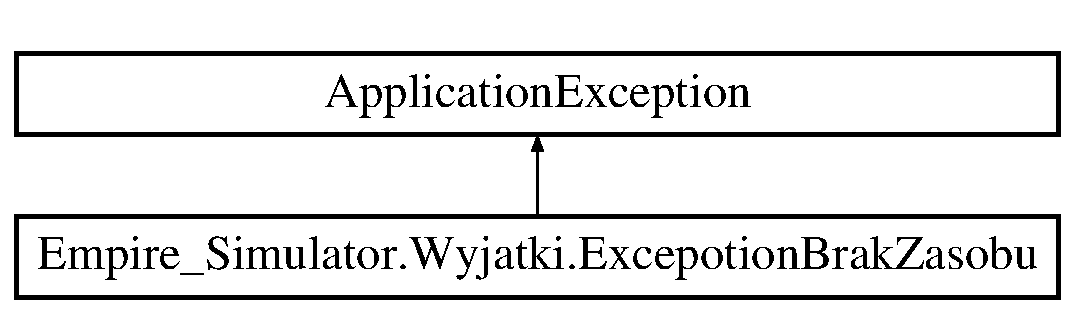
\includegraphics[height=2.000000cm]{class_empire___simulator_1_1_wyjatki_1_1_excepotion_brak_zasobu}
\end{center}
\end{figure}


The documentation for this class was generated from the following file\+:\begin{DoxyCompactItemize}
\item 
C\+:/\+Users/\+Paweł/\+Documents/\+Git\+Hub/\+Empire\+\_\+\+Simulator\+\_\+\+V\+S\+\_\+2008/\+Empire\+\_\+\+Simulator/\+Empire\+\_\+\+Simulator/\+Wyjatki/Excepotion\+Brak\+Zasobu.\+cs\end{DoxyCompactItemize}

\hypertarget{class_empire___simulator_1_1_fabryka_handlarzy}{\section{Empire\+\_\+\+Simulator.\+Fabryka\+Handlarzy Class Reference}
\label{class_empire___simulator_1_1_fabryka_handlarzy}\index{Empire\+\_\+\+Simulator.\+Fabryka\+Handlarzy@{Empire\+\_\+\+Simulator.\+Fabryka\+Handlarzy}}
}


generuje handlarzy z podana strategią i iloscia towaru ktora mogą ze sobą wozić.  


\subsection*{Public Member Functions}
\begin{DoxyCompactItemize}
\item 
\hypertarget{class_empire___simulator_1_1_fabryka_handlarzy_ac57e9502961d8f7713b1071c8557387a}{{\bfseries Fabryka\+Handlarzy} (int ladownosc)}\label{class_empire___simulator_1_1_fabryka_handlarzy_ac57e9502961d8f7713b1071c8557387a}

\item 
\hypertarget{class_empire___simulator_1_1_fabryka_handlarzy_a1526a5d274fa0c33722422a98de43644}{\hyperlink{class_empire___simulator_1_1_handlarz}{Handlarz} {\bfseries generuj\+Handlarza} ()}\label{class_empire___simulator_1_1_fabryka_handlarzy_a1526a5d274fa0c33722422a98de43644}

\end{DoxyCompactItemize}


\subsection{Detailed Description}
generuje handlarzy z podana strategią i iloscia towaru ktora mogą ze sobą wozić. 



The documentation for this class was generated from the following file\+:\begin{DoxyCompactItemize}
\item 
C\+:/\+Users/\+Paweł/\+Documents/\+Git\+Hub/\+Empire\+\_\+\+Simulator\+\_\+\+V\+S\+\_\+2008/\+Empire\+\_\+\+Simulator/\+Empire\+\_\+\+Simulator/\+Klasy/\+Handlarz/Fabryka\+Handlarzy.\+cs\end{DoxyCompactItemize}

\hypertarget{class_empire___simulator_1_1_fabryka_osad}{\section{Empire\+\_\+\+Simulator.\+Fabryka\+Osad Class Reference}
\label{class_empire___simulator_1_1_fabryka_osad}\index{Empire\+\_\+\+Simulator.\+Fabryka\+Osad@{Empire\+\_\+\+Simulator.\+Fabryka\+Osad}}
}


Klasa która tworzy Osady  


\subsection*{Public Member Functions}
\begin{DoxyCompactItemize}
\item 
\hypertarget{class_empire___simulator_1_1_fabryka_osad_ab4272a59d8ad30440880bfc2dabe4c46}{{\bfseries Fabryka\+Osad} (\hyperlink{class_empire___simulator_1_1_fabryka_zasobow}{Fabryka\+Zasobow} fabryka\+Zasobow, \hyperlink{interface_empire___simulator_1_1_i_strategia_osady}{I\+Strategia\+Osady} strategia\+Osady, \hyperlink{interface_empire___simulator_1_1_i_strategia_handlu}{I\+Strategia\+Handlu} strategia\+Handlu)}\label{class_empire___simulator_1_1_fabryka_osad_ab4272a59d8ad30440880bfc2dabe4c46}

\item 
\hyperlink{class_empire___simulator_1_1_osada}{Osada} \hyperlink{class_empire___simulator_1_1_fabryka_osad_a367b4c78f10a1b2c632813294a0e5d2f}{losuj\+Osade} ()
\begin{DoxyCompactList}\small\item\em Losuje osadę \end{DoxyCompactList}\end{DoxyCompactItemize}


\subsection{Detailed Description}
Klasa która tworzy Osady 



\subsection{Member Function Documentation}
\hypertarget{class_empire___simulator_1_1_fabryka_osad_a367b4c78f10a1b2c632813294a0e5d2f}{\index{Empire\+\_\+\+Simulator\+::\+Fabryka\+Osad@{Empire\+\_\+\+Simulator\+::\+Fabryka\+Osad}!losuj\+Osade@{losuj\+Osade}}
\index{losuj\+Osade@{losuj\+Osade}!Empire\+\_\+\+Simulator\+::\+Fabryka\+Osad@{Empire\+\_\+\+Simulator\+::\+Fabryka\+Osad}}
\subsubsection[{losuj\+Osade}]{\setlength{\rightskip}{0pt plus 5cm}{\bf Osada} Empire\+\_\+\+Simulator.\+Fabryka\+Osad.\+losuj\+Osade (
\begin{DoxyParamCaption}
{}
\end{DoxyParamCaption}
)\hspace{0.3cm}{\ttfamily [inline]}}}\label{class_empire___simulator_1_1_fabryka_osad_a367b4c78f10a1b2c632813294a0e5d2f}


Losuje osadę 

\begin{DoxyReturn}{Returns}
konkretny gotowy do użytku obiekt typu osada
\end{DoxyReturn}


The documentation for this class was generated from the following file\+:\begin{DoxyCompactItemize}
\item 
C\+:/\+Users/\+Paweł/\+Documents/\+Git\+Hub/\+Empire\+\_\+\+Simulator\+\_\+\+V\+S\+\_\+2008/\+Empire\+\_\+\+Simulator/\+Empire\+\_\+\+Simulator/\+Klasy/\+Osada/Fabryka\+Osad.\+cs\end{DoxyCompactItemize}

\hypertarget{class_empire___simulator_1_1_fabryka_zasobow}{\section{Empire\+\_\+\+Simulator.\+Fabryka\+Zasobow Class Reference}
\label{class_empire___simulator_1_1_fabryka_zasobow}\index{Empire\+\_\+\+Simulator.\+Fabryka\+Zasobow@{Empire\+\_\+\+Simulator.\+Fabryka\+Zasobow}}
}


Fabryka Zasobow to klasa ktora potrafi generowac gotowe do uzycia obiekty zasobow na podstawie swoich danyh  


\subsection*{Public Member Functions}
\begin{DoxyCompactItemize}
\item 
List$<$ \hyperlink{class_empire___simulator_1_1_zasob}{Zasob} $>$ \hyperlink{class_empire___simulator_1_1_fabryka_zasobow_a3fb3f39dd352878a2131ac7cedea0f29}{tworzenie\+Zasobow} ()
\begin{DoxyCompactList}\small\item\em Tworzy tyle obiektow zasobu ile jest nazw w liscie utworzonych nazw zasobow i umieszcza je na liscie dzieki temu uzywajac pozniej takiej fabryki wiemy ze dostaniemy liste obiektow na ktorej znadzie sie obiekt kazdego z zasobow dostepnych w grze \end{DoxyCompactList}\item 
List$<$ string $>$ \hyperlink{class_empire___simulator_1_1_fabryka_zasobow_a4a16809482dea3984053434ccc065769}{lista\+Zasobow} ()
\begin{DoxyCompactList}\small\item\em zwraca liste ktorej uzywa losowanie potencjalu \end{DoxyCompactList}\end{DoxyCompactItemize}


\subsection{Detailed Description}
Fabryka Zasobow to klasa ktora potrafi generowac gotowe do uzycia obiekty zasobow na podstawie swoich danyh 



\subsection{Member Function Documentation}
\hypertarget{class_empire___simulator_1_1_fabryka_zasobow_a4a16809482dea3984053434ccc065769}{\index{Empire\+\_\+\+Simulator\+::\+Fabryka\+Zasobow@{Empire\+\_\+\+Simulator\+::\+Fabryka\+Zasobow}!lista\+Zasobow@{lista\+Zasobow}}
\index{lista\+Zasobow@{lista\+Zasobow}!Empire\+\_\+\+Simulator\+::\+Fabryka\+Zasobow@{Empire\+\_\+\+Simulator\+::\+Fabryka\+Zasobow}}
\subsubsection[{lista\+Zasobow}]{\setlength{\rightskip}{0pt plus 5cm}List$<$string$>$ Empire\+\_\+\+Simulator.\+Fabryka\+Zasobow.\+lista\+Zasobow (
\begin{DoxyParamCaption}
{}
\end{DoxyParamCaption}
)\hspace{0.3cm}{\ttfamily [inline]}}}\label{class_empire___simulator_1_1_fabryka_zasobow_a4a16809482dea3984053434ccc065769}


zwraca liste ktorej uzywa losowanie potencjalu 

\begin{DoxyReturn}{Returns}

\end{DoxyReturn}
\hypertarget{class_empire___simulator_1_1_fabryka_zasobow_a3fb3f39dd352878a2131ac7cedea0f29}{\index{Empire\+\_\+\+Simulator\+::\+Fabryka\+Zasobow@{Empire\+\_\+\+Simulator\+::\+Fabryka\+Zasobow}!tworzenie\+Zasobow@{tworzenie\+Zasobow}}
\index{tworzenie\+Zasobow@{tworzenie\+Zasobow}!Empire\+\_\+\+Simulator\+::\+Fabryka\+Zasobow@{Empire\+\_\+\+Simulator\+::\+Fabryka\+Zasobow}}
\subsubsection[{tworzenie\+Zasobow}]{\setlength{\rightskip}{0pt plus 5cm}List$<${\bf Zasob}$>$ Empire\+\_\+\+Simulator.\+Fabryka\+Zasobow.\+tworzenie\+Zasobow (
\begin{DoxyParamCaption}
{}
\end{DoxyParamCaption}
)\hspace{0.3cm}{\ttfamily [inline]}}}\label{class_empire___simulator_1_1_fabryka_zasobow_a3fb3f39dd352878a2131ac7cedea0f29}


Tworzy tyle obiektow zasobu ile jest nazw w liscie utworzonych nazw zasobow i umieszcza je na liscie dzieki temu uzywajac pozniej takiej fabryki wiemy ze dostaniemy liste obiektow na ktorej znadzie sie obiekt kazdego z zasobow dostepnych w grze 

\begin{DoxyReturn}{Returns}
lista konkretnych gotowych obiektow typu zasób
\end{DoxyReturn}


The documentation for this class was generated from the following file\+:\begin{DoxyCompactItemize}
\item 
C\+:/\+Users/\+Paweł/\+Documents/\+Git\+Hub/\+Empire\+\_\+\+Simulator\+\_\+\+V\+S\+\_\+2008/\+Empire\+\_\+\+Simulator/\+Empire\+\_\+\+Simulator/\+Klasy/\+Zasob/Fabryka\+Zasobow.\+cs\end{DoxyCompactItemize}

\hypertarget{class_empire___simulator_1_1_generator_mapy}{\section{Empire\+\_\+\+Simulator.\+Generator\+Mapy Class Reference}
\label{class_empire___simulator_1_1_generator_mapy}\index{Empire\+\_\+\+Simulator.\+Generator\+Mapy@{Empire\+\_\+\+Simulator.\+Generator\+Mapy}}
}


Obiekt generatora mapy pozwala na naniesienie osad,handlarzy i tła na ramkę gry  


\subsection*{Public Member Functions}
\begin{DoxyCompactItemize}
\item 
\hypertarget{class_empire___simulator_1_1_generator_mapy_a7bd64ecdfb35d65f5f87755533562ce7}{void {\bfseries generuj\+Mape} (\hyperlink{class_empire___simulator_1_1_okno_gry}{Okno\+Gry} okno, \hyperlink{class_empire___simulator_1_1_swiat}{Swiat} swiat)}\label{class_empire___simulator_1_1_generator_mapy_a7bd64ecdfb35d65f5f87755533562ce7}

\item 
\hyperlink{class_empire___simulator_1_1_aktualizator_mapy}{Aktualizator\+Mapy} \hyperlink{class_empire___simulator_1_1_generator_mapy_a0c22f0b317eae838c2e15f5baaa1fa31}{generuj\+Aktualizatora\+Mapy} ()
\begin{DoxyCompactList}\small\item\em na podstawie mapy generuje obiekt jej aktualizatora \end{DoxyCompactList}\end{DoxyCompactItemize}


\subsection{Detailed Description}
Obiekt generatora mapy pozwala na naniesienie osad,handlarzy i tła na ramkę gry 



\subsection{Member Function Documentation}
\hypertarget{class_empire___simulator_1_1_generator_mapy_a0c22f0b317eae838c2e15f5baaa1fa31}{\index{Empire\+\_\+\+Simulator\+::\+Generator\+Mapy@{Empire\+\_\+\+Simulator\+::\+Generator\+Mapy}!generuj\+Aktualizatora\+Mapy@{generuj\+Aktualizatora\+Mapy}}
\index{generuj\+Aktualizatora\+Mapy@{generuj\+Aktualizatora\+Mapy}!Empire\+\_\+\+Simulator\+::\+Generator\+Mapy@{Empire\+\_\+\+Simulator\+::\+Generator\+Mapy}}
\subsubsection[{generuj\+Aktualizatora\+Mapy}]{\setlength{\rightskip}{0pt plus 5cm}{\bf Aktualizator\+Mapy} Empire\+\_\+\+Simulator.\+Generator\+Mapy.\+generuj\+Aktualizatora\+Mapy (
\begin{DoxyParamCaption}
{}
\end{DoxyParamCaption}
)\hspace{0.3cm}{\ttfamily [inline]}}}\label{class_empire___simulator_1_1_generator_mapy_a0c22f0b317eae838c2e15f5baaa1fa31}


na podstawie mapy generuje obiekt jej aktualizatora 

\begin{DoxyReturn}{Returns}

\end{DoxyReturn}


The documentation for this class was generated from the following file\+:\begin{DoxyCompactItemize}
\item 
C\+:/\+Users/\+Paweł/\+Documents/\+Git\+Hub/\+Empire\+\_\+\+Simulator\+\_\+\+V\+S\+\_\+2008/\+Empire\+\_\+\+Simulator/\+Empire\+\_\+\+Simulator/\+Mapa/Generator\+Mapy.\+cs\end{DoxyCompactItemize}

\hypertarget{class_empire___simulator_1_1_generator_swiata}{\section{Empire\+\_\+\+Simulator.\+Generator\+Swiata Class Reference}
\label{class_empire___simulator_1_1_generator_swiata}\index{Empire\+\_\+\+Simulator.\+Generator\+Swiata@{Empire\+\_\+\+Simulator.\+Generator\+Swiata}}
}


Jest to klasa której obiekt potrafi wygenerowac swiat na podstawie podanej strategi  


\subsection*{Public Member Functions}
\begin{DoxyCompactItemize}
\item 
\hyperlink{class_empire___simulator_1_1_swiat}{Swiat} \hyperlink{class_empire___simulator_1_1_generator_swiata_af7f2f847587df138e2bbd13f7b84064b}{generuj\+Swiat} ()
\begin{DoxyCompactList}\small\item\em zwraca wygenerowany Świat \end{DoxyCompactList}\end{DoxyCompactItemize}


\subsection{Detailed Description}
Jest to klasa której obiekt potrafi wygenerowac swiat na podstawie podanej strategi 



\subsection{Member Function Documentation}
\hypertarget{class_empire___simulator_1_1_generator_swiata_af7f2f847587df138e2bbd13f7b84064b}{\index{Empire\+\_\+\+Simulator\+::\+Generator\+Swiata@{Empire\+\_\+\+Simulator\+::\+Generator\+Swiata}!generuj\+Swiat@{generuj\+Swiat}}
\index{generuj\+Swiat@{generuj\+Swiat}!Empire\+\_\+\+Simulator\+::\+Generator\+Swiata@{Empire\+\_\+\+Simulator\+::\+Generator\+Swiata}}
\subsubsection[{generuj\+Swiat}]{\setlength{\rightskip}{0pt plus 5cm}{\bf Swiat} Empire\+\_\+\+Simulator.\+Generator\+Swiata.\+generuj\+Swiat (
\begin{DoxyParamCaption}
{}
\end{DoxyParamCaption}
)\hspace{0.3cm}{\ttfamily [inline]}}}\label{class_empire___simulator_1_1_generator_swiata_af7f2f847587df138e2bbd13f7b84064b}


zwraca wygenerowany Świat 

\begin{DoxyReturn}{Returns}
Obekt klasy Świat
\end{DoxyReturn}


The documentation for this class was generated from the following file\+:\begin{DoxyCompactItemize}
\item 
C\+:/\+Users/\+Paweł/\+Documents/\+Git\+Hub/\+Empire\+\_\+\+Simulator\+\_\+\+V\+S\+\_\+2008/\+Empire\+\_\+\+Simulator/\+Empire\+\_\+\+Simulator/\+Klasy/\+Swiat/Generator\+Swiata.\+cs\end{DoxyCompactItemize}

\hypertarget{class_empire___simulator_1_1_handlarz}{\section{Empire\+\_\+\+Simulator.\+Handlarz Class Reference}
\label{class_empire___simulator_1_1_handlarz}\index{Empire\+\_\+\+Simulator.\+Handlarz@{Empire\+\_\+\+Simulator.\+Handlarz}}
}
\subsection*{Public Member Functions}
\begin{DoxyCompactItemize}
\item 
\hypertarget{class_empire___simulator_1_1_handlarz_a7ea63718304e5484b7526e0e3f154941}{{\bfseries Handlarz} (int ladownosc\+Wozu, string nazwa)}\label{class_empire___simulator_1_1_handlarz_a7ea63718304e5484b7526e0e3f154941}

\item 
\hypertarget{class_empire___simulator_1_1_handlarz_a8b1f29aed34339e6136739184e4faa89}{void {\bfseries ustal\+Strategie} (\hyperlink{interface_empire___simulator_1_1_i_strategia_handlarza}{I\+Strategia\+Handlarza} strategia)}\label{class_empire___simulator_1_1_handlarz_a8b1f29aed34339e6136739184e4faa89}

\item 
\hyperlink{class_empire___simulator_1_1_osada}{Osada} \hyperlink{class_empire___simulator_1_1_handlarz_a2257fab877e2c0362adfea97823c09f4}{Wyznacz\+Cel\+Podrozy} ()
\begin{DoxyCompactList}\small\item\em Wyznacza cel podróży na podstawie tego co ma na wozie i strategi handlarza \end{DoxyCompactList}\item 
\hyperlink{class_empire___simulator_1_1_woz_handlarza}{Woz\+Handlarza} \hyperlink{class_empire___simulator_1_1_handlarz_aabded215d71b5fbcfec11027a8bf4593}{zwroc\+Woz} ()
\begin{DoxyCompactList}\small\item\em Zwraca to co ma na wozie (Czy to napewno dobry pomysl?) lepiej chyba bedzie jesli kazda kominikacja z wozem bedzie odbywala sie za pomoca handlarza \end{DoxyCompactList}\item 
Key\+Value\+Pair$<$ string, \hyperlink{class_empire___simulator_1_1_zasob}{Zasob} $>$ \hyperlink{class_empire___simulator_1_1_handlarz_a4c3a0bb8e7fcbaf374c42c70c0979b29}{rozladuj\+Towar} ()
\begin{DoxyCompactList}\small\item\em rozladowuje towar ze swjojego wozu \end{DoxyCompactList}\item 
void \hyperlink{class_empire___simulator_1_1_handlarz_adc85cfddd7e9edf1aa2eaaa064e765c9}{laduj\+Towar} (Key\+Value\+Pair$<$ string, \hyperlink{class_empire___simulator_1_1_zasob}{Zasob} $>$ towar)
\begin{DoxyCompactList}\small\item\em laduje dany towar na woz i ustala sobie na podstawie tego co zaladowal nowy cel podróży. \end{DoxyCompactList}\item 
Point \hyperlink{class_empire___simulator_1_1_handlarz_ae6c1178490e2a429ece397f5b3a656d9}{zwroc\+Pozycje} ()
\begin{DoxyCompactList}\small\item\em zwraca pozycje w jakiej znajduje się handlarz \end{DoxyCompactList}\item 
void \hyperlink{class_empire___simulator_1_1_handlarz_a1d1c6dbfb9b01f787a5bd2d87ff2011b}{aktualizuj} ()
\begin{DoxyCompactList}\small\item\em Aktualizuje stan handlarza przesuwa go do nowej pozyjci i ew wsyła na targ jesli jest blisko osady \end{DoxyCompactList}\item 
\hyperlink{class_empire___simulator_1_1_osada}{Osada} \hyperlink{class_empire___simulator_1_1_handlarz_ad51b2b7a3552a81ee97a2e56d8c2b4a9}{zwroc\+Cel\+Podrozy} ()
\begin{DoxyCompactList}\small\item\em zwraca do jakiej osady podróżuje handlarz \end{DoxyCompactList}\item 
\hypertarget{class_empire___simulator_1_1_handlarz_afa89dc166094616e01884c0d014edbb2}{override string {\bfseries To\+String} ()}\label{class_empire___simulator_1_1_handlarz_afa89dc166094616e01884c0d014edbb2}

\item 
\hypertarget{class_empire___simulator_1_1_handlarz_a01ce9c16678c486a0d62d331b7fff939}{void {\bfseries reczne\+Ustawienie\+Celu} (\hyperlink{class_empire___simulator_1_1_osada}{Osada} osada)}\label{class_empire___simulator_1_1_handlarz_a01ce9c16678c486a0d62d331b7fff939}

\end{DoxyCompactItemize}


\subsection{Member Function Documentation}
\hypertarget{class_empire___simulator_1_1_handlarz_a1d1c6dbfb9b01f787a5bd2d87ff2011b}{\index{Empire\+\_\+\+Simulator\+::\+Handlarz@{Empire\+\_\+\+Simulator\+::\+Handlarz}!aktualizuj@{aktualizuj}}
\index{aktualizuj@{aktualizuj}!Empire\+\_\+\+Simulator\+::\+Handlarz@{Empire\+\_\+\+Simulator\+::\+Handlarz}}
\subsubsection[{aktualizuj}]{\setlength{\rightskip}{0pt plus 5cm}void Empire\+\_\+\+Simulator.\+Handlarz.\+aktualizuj (
\begin{DoxyParamCaption}
{}
\end{DoxyParamCaption}
)\hspace{0.3cm}{\ttfamily [inline]}}}\label{class_empire___simulator_1_1_handlarz_a1d1c6dbfb9b01f787a5bd2d87ff2011b}


Aktualizuje stan handlarza przesuwa go do nowej pozyjci i ew wsyła na targ jesli jest blisko osady 

\hypertarget{class_empire___simulator_1_1_handlarz_adc85cfddd7e9edf1aa2eaaa064e765c9}{\index{Empire\+\_\+\+Simulator\+::\+Handlarz@{Empire\+\_\+\+Simulator\+::\+Handlarz}!laduj\+Towar@{laduj\+Towar}}
\index{laduj\+Towar@{laduj\+Towar}!Empire\+\_\+\+Simulator\+::\+Handlarz@{Empire\+\_\+\+Simulator\+::\+Handlarz}}
\subsubsection[{laduj\+Towar}]{\setlength{\rightskip}{0pt plus 5cm}void Empire\+\_\+\+Simulator.\+Handlarz.\+laduj\+Towar (
\begin{DoxyParamCaption}
\item[{Key\+Value\+Pair$<$ string, {\bf Zasob} $>$}]{towar}
\end{DoxyParamCaption}
)\hspace{0.3cm}{\ttfamily [inline]}}}\label{class_empire___simulator_1_1_handlarz_adc85cfddd7e9edf1aa2eaaa064e765c9}


laduje dany towar na woz i ustala sobie na podstawie tego co zaladowal nowy cel podróży. 


\begin{DoxyParams}{Parameters}
{\em towar} & \\
\hline
\end{DoxyParams}
\hypertarget{class_empire___simulator_1_1_handlarz_a4c3a0bb8e7fcbaf374c42c70c0979b29}{\index{Empire\+\_\+\+Simulator\+::\+Handlarz@{Empire\+\_\+\+Simulator\+::\+Handlarz}!rozladuj\+Towar@{rozladuj\+Towar}}
\index{rozladuj\+Towar@{rozladuj\+Towar}!Empire\+\_\+\+Simulator\+::\+Handlarz@{Empire\+\_\+\+Simulator\+::\+Handlarz}}
\subsubsection[{rozladuj\+Towar}]{\setlength{\rightskip}{0pt plus 5cm}Key\+Value\+Pair$<$string, {\bf Zasob}$>$ Empire\+\_\+\+Simulator.\+Handlarz.\+rozladuj\+Towar (
\begin{DoxyParamCaption}
{}
\end{DoxyParamCaption}
)\hspace{0.3cm}{\ttfamily [inline]}}}\label{class_empire___simulator_1_1_handlarz_a4c3a0bb8e7fcbaf374c42c70c0979b29}


rozladowuje towar ze swjojego wozu 

\begin{DoxyReturn}{Returns}
para nazwy zasobu z zasobem
\end{DoxyReturn}
\hypertarget{class_empire___simulator_1_1_handlarz_a2257fab877e2c0362adfea97823c09f4}{\index{Empire\+\_\+\+Simulator\+::\+Handlarz@{Empire\+\_\+\+Simulator\+::\+Handlarz}!Wyznacz\+Cel\+Podrozy@{Wyznacz\+Cel\+Podrozy}}
\index{Wyznacz\+Cel\+Podrozy@{Wyznacz\+Cel\+Podrozy}!Empire\+\_\+\+Simulator\+::\+Handlarz@{Empire\+\_\+\+Simulator\+::\+Handlarz}}
\subsubsection[{Wyznacz\+Cel\+Podrozy}]{\setlength{\rightskip}{0pt plus 5cm}{\bf Osada} Empire\+\_\+\+Simulator.\+Handlarz.\+Wyznacz\+Cel\+Podrozy (
\begin{DoxyParamCaption}
{}
\end{DoxyParamCaption}
)\hspace{0.3cm}{\ttfamily [inline]}}}\label{class_empire___simulator_1_1_handlarz_a2257fab877e2c0362adfea97823c09f4}


Wyznacza cel podróży na podstawie tego co ma na wozie i strategi handlarza 

\begin{DoxyReturn}{Returns}
obiekt osady do ktorej sie kieruje
\end{DoxyReturn}
\hypertarget{class_empire___simulator_1_1_handlarz_ad51b2b7a3552a81ee97a2e56d8c2b4a9}{\index{Empire\+\_\+\+Simulator\+::\+Handlarz@{Empire\+\_\+\+Simulator\+::\+Handlarz}!zwroc\+Cel\+Podrozy@{zwroc\+Cel\+Podrozy}}
\index{zwroc\+Cel\+Podrozy@{zwroc\+Cel\+Podrozy}!Empire\+\_\+\+Simulator\+::\+Handlarz@{Empire\+\_\+\+Simulator\+::\+Handlarz}}
\subsubsection[{zwroc\+Cel\+Podrozy}]{\setlength{\rightskip}{0pt plus 5cm}{\bf Osada} Empire\+\_\+\+Simulator.\+Handlarz.\+zwroc\+Cel\+Podrozy (
\begin{DoxyParamCaption}
{}
\end{DoxyParamCaption}
)\hspace{0.3cm}{\ttfamily [inline]}}}\label{class_empire___simulator_1_1_handlarz_ad51b2b7a3552a81ee97a2e56d8c2b4a9}


zwraca do jakiej osady podróżuje handlarz 

\begin{DoxyReturn}{Returns}
obiekt osady
\end{DoxyReturn}
\hypertarget{class_empire___simulator_1_1_handlarz_ae6c1178490e2a429ece397f5b3a656d9}{\index{Empire\+\_\+\+Simulator\+::\+Handlarz@{Empire\+\_\+\+Simulator\+::\+Handlarz}!zwroc\+Pozycje@{zwroc\+Pozycje}}
\index{zwroc\+Pozycje@{zwroc\+Pozycje}!Empire\+\_\+\+Simulator\+::\+Handlarz@{Empire\+\_\+\+Simulator\+::\+Handlarz}}
\subsubsection[{zwroc\+Pozycje}]{\setlength{\rightskip}{0pt plus 5cm}Point Empire\+\_\+\+Simulator.\+Handlarz.\+zwroc\+Pozycje (
\begin{DoxyParamCaption}
{}
\end{DoxyParamCaption}
)\hspace{0.3cm}{\ttfamily [inline]}}}\label{class_empire___simulator_1_1_handlarz_ae6c1178490e2a429ece397f5b3a656d9}


zwraca pozycje w jakiej znajduje się handlarz 

\begin{DoxyReturn}{Returns}
Point(\+X,\+Y)
\end{DoxyReturn}
\hypertarget{class_empire___simulator_1_1_handlarz_aabded215d71b5fbcfec11027a8bf4593}{\index{Empire\+\_\+\+Simulator\+::\+Handlarz@{Empire\+\_\+\+Simulator\+::\+Handlarz}!zwroc\+Woz@{zwroc\+Woz}}
\index{zwroc\+Woz@{zwroc\+Woz}!Empire\+\_\+\+Simulator\+::\+Handlarz@{Empire\+\_\+\+Simulator\+::\+Handlarz}}
\subsubsection[{zwroc\+Woz}]{\setlength{\rightskip}{0pt plus 5cm}{\bf Woz\+Handlarza} Empire\+\_\+\+Simulator.\+Handlarz.\+zwroc\+Woz (
\begin{DoxyParamCaption}
{}
\end{DoxyParamCaption}
)\hspace{0.3cm}{\ttfamily [inline]}}}\label{class_empire___simulator_1_1_handlarz_aabded215d71b5fbcfec11027a8bf4593}


Zwraca to co ma na wozie (Czy to napewno dobry pomysl?) lepiej chyba bedzie jesli kazda kominikacja z wozem bedzie odbywala sie za pomoca handlarza 

\begin{DoxyReturn}{Returns}
obiekt wozu handlarza
\end{DoxyReturn}


The documentation for this class was generated from the following file\+:\begin{DoxyCompactItemize}
\item 
C\+:/\+Users/\+Paweł/\+Documents/\+Git\+Hub/\+Empire\+\_\+\+Simulator\+\_\+\+V\+S\+\_\+2008/\+Empire\+\_\+\+Simulator/\+Empire\+\_\+\+Simulator/\+Klasy/\+Handlarz/Handlarz.\+cs\end{DoxyCompactItemize}

\hypertarget{interface_empire___simulator_1_1_i_strategia_aktualizacji_swiata}{\section{Empire\+\_\+\+Simulator.\+I\+Strategia\+Aktualizacji\+Swiata Interface Reference}
\label{interface_empire___simulator_1_1_i_strategia_aktualizacji_swiata}\index{Empire\+\_\+\+Simulator.\+I\+Strategia\+Aktualizacji\+Swiata@{Empire\+\_\+\+Simulator.\+I\+Strategia\+Aktualizacji\+Swiata}}
}


Interfejs Aktualizacji swiata ma metody zwracajace to co ile dni handlarz zmienia swój stan, podobnie tyczy się to wioski  


Inheritance diagram for Empire\+\_\+\+Simulator.\+I\+Strategia\+Aktualizacji\+Swiata\+:\begin{figure}[H]
\begin{center}
\leavevmode
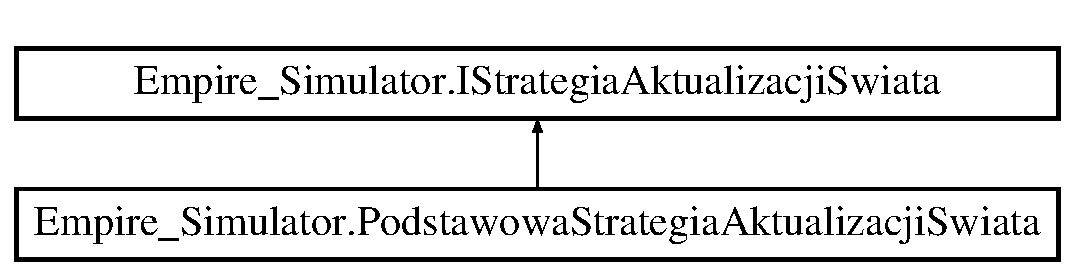
\includegraphics[height=2.000000cm]{interface_empire___simulator_1_1_i_strategia_aktualizacji_swiata}
\end{center}
\end{figure}
\subsection*{Public Member Functions}
\begin{DoxyCompactItemize}
\item 
\hypertarget{interface_empire___simulator_1_1_i_strategia_aktualizacji_swiata_a449765a9f768f9a3a4412aff2f1a2b51}{int {\bfseries co\+Ile\+Dni\+Aktualizowac\+Osade} ()}\label{interface_empire___simulator_1_1_i_strategia_aktualizacji_swiata_a449765a9f768f9a3a4412aff2f1a2b51}

\item 
\hypertarget{interface_empire___simulator_1_1_i_strategia_aktualizacji_swiata_a2378bb4f6e915e985e7dfbeb8d9662ec}{int {\bfseries co\+Ile\+Dni\+Aktualizowac\+Handlarza} ()}\label{interface_empire___simulator_1_1_i_strategia_aktualizacji_swiata_a2378bb4f6e915e985e7dfbeb8d9662ec}

\end{DoxyCompactItemize}


\subsection{Detailed Description}
Interfejs Aktualizacji swiata ma metody zwracajace to co ile dni handlarz zmienia swój stan, podobnie tyczy się to wioski 



The documentation for this interface was generated from the following file\+:\begin{DoxyCompactItemize}
\item 
C\+:/\+Users/\+Paweł/\+Documents/\+Git\+Hub/\+Empire\+\_\+\+Simulator\+\_\+\+V\+S\+\_\+2008/\+Empire\+\_\+\+Simulator/\+Empire\+\_\+\+Simulator/\+Interfejsy/I\+Strategia\+Aktualizacji\+Swiata.\+cs\end{DoxyCompactItemize}

\hypertarget{interface_empire___simulator_1_1_i_strategia_generowania_swiata}{\section{Empire\+\_\+\+Simulator.\+I\+Strategia\+Generowania\+Swiata Interface Reference}
\label{interface_empire___simulator_1_1_i_strategia_generowania_swiata}\index{Empire\+\_\+\+Simulator.\+I\+Strategia\+Generowania\+Swiata@{Empire\+\_\+\+Simulator.\+I\+Strategia\+Generowania\+Swiata}}
}


Jest to ogolny interfejs generowania swiata, ktory mówi o tym ile osad wygenerowac na mapie, ilu handlarzy,i jaka pojemność bedzie miał wóz handlarze podaje też z jakich strategi handlarza,handlu i Osady bedziemy korzystac  


Inheritance diagram for Empire\+\_\+\+Simulator.\+I\+Strategia\+Generowania\+Swiata\+:\begin{figure}[H]
\begin{center}
\leavevmode
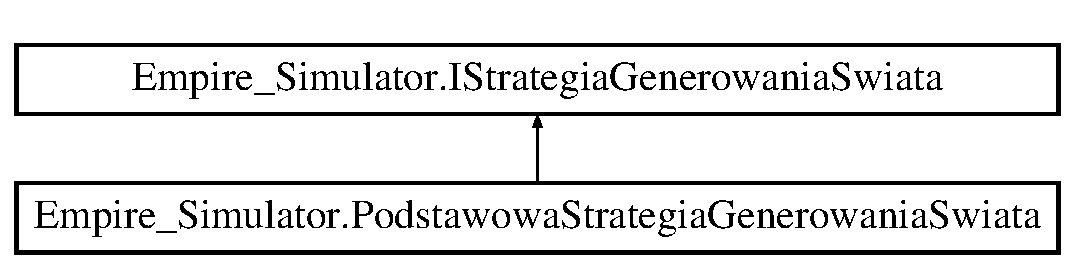
\includegraphics[height=2.000000cm]{interface_empire___simulator_1_1_i_strategia_generowania_swiata}
\end{center}
\end{figure}
\subsection*{Public Member Functions}
\begin{DoxyCompactItemize}
\item 
\hypertarget{interface_empire___simulator_1_1_i_strategia_generowania_swiata_ae12937c8cec1dd6cfb64be80ef07ebff}{int {\bfseries ilosc\+Osad\+Do\+Wygenerowania} ()}\label{interface_empire___simulator_1_1_i_strategia_generowania_swiata_ae12937c8cec1dd6cfb64be80ef07ebff}

\item 
\hypertarget{interface_empire___simulator_1_1_i_strategia_generowania_swiata_a8145d4a98b2395911e7bb4d85384b284}{int {\bfseries ilosc\+Handlarzy\+Do\+Wygenerowania} ()}\label{interface_empire___simulator_1_1_i_strategia_generowania_swiata_a8145d4a98b2395911e7bb4d85384b284}

\item 
\hypertarget{interface_empire___simulator_1_1_i_strategia_generowania_swiata_aa37c357c667724f86037976d00da07cc}{int {\bfseries pojemnosc\+Wozu\+Handlarza} ()}\label{interface_empire___simulator_1_1_i_strategia_generowania_swiata_aa37c357c667724f86037976d00da07cc}

\item 
\hypertarget{interface_empire___simulator_1_1_i_strategia_generowania_swiata_a1170bcc5bb31bdda8f2be28d7c69cc1b}{\hyperlink{interface_empire___simulator_1_1_i_strategia_handlarza}{I\+Strategia\+Handlarza} {\bfseries strategia\+Handlarza} (List$<$ \hyperlink{class_empire___simulator_1_1_osada}{Osada} $>$ lista\+Osad, List$<$ \hyperlink{class_empire___simulator_1_1_handlarz}{Handlarz} $>$ lista\+Handlarzy)}\label{interface_empire___simulator_1_1_i_strategia_generowania_swiata_a1170bcc5bb31bdda8f2be28d7c69cc1b}

\item 
\hypertarget{interface_empire___simulator_1_1_i_strategia_generowania_swiata_ae2d930bea01b0777b605749cad794dcc}{\hyperlink{interface_empire___simulator_1_1_i_strategia_handlu}{I\+Strategia\+Handlu} {\bfseries strategia\+Handlu} ()}\label{interface_empire___simulator_1_1_i_strategia_generowania_swiata_ae2d930bea01b0777b605749cad794dcc}

\item 
\hypertarget{interface_empire___simulator_1_1_i_strategia_generowania_swiata_abc39873591ff95bde54ba028e9c7f55b}{\hyperlink{interface_empire___simulator_1_1_i_strategia_osady}{I\+Strategia\+Osady} {\bfseries strategia\+Osady} ()}\label{interface_empire___simulator_1_1_i_strategia_generowania_swiata_abc39873591ff95bde54ba028e9c7f55b}

\end{DoxyCompactItemize}


\subsection{Detailed Description}
Jest to ogolny interfejs generowania swiata, ktory mówi o tym ile osad wygenerowac na mapie, ilu handlarzy,i jaka pojemność bedzie miał wóz handlarze podaje też z jakich strategi handlarza,handlu i Osady bedziemy korzystac 



The documentation for this interface was generated from the following file\+:\begin{DoxyCompactItemize}
\item 
C\+:/\+Users/\+Paweł/\+Documents/\+Git\+Hub/\+Empire\+\_\+\+Simulator\+\_\+\+V\+S\+\_\+2008/\+Empire\+\_\+\+Simulator/\+Empire\+\_\+\+Simulator/\+Interfejsy/I\+Strategia\+Generowania\+Swiata.\+cs\end{DoxyCompactItemize}

\hypertarget{interface_empire___simulator_1_1_i_strategia_handlarza}{\section{Empire\+\_\+\+Simulator.\+I\+Strategia\+Handlarza Interface Reference}
\label{interface_empire___simulator_1_1_i_strategia_handlarza}\index{Empire\+\_\+\+Simulator.\+I\+Strategia\+Handlarza@{Empire\+\_\+\+Simulator.\+I\+Strategia\+Handlarza}}
}


Interfejs mówiący o tym jak wyznaczać nowy cel podróży dla handlarza oraz w jaki sposob sie przemieszcza  


Inheritance diagram for Empire\+\_\+\+Simulator.\+I\+Strategia\+Handlarza\+:\begin{figure}[H]
\begin{center}
\leavevmode
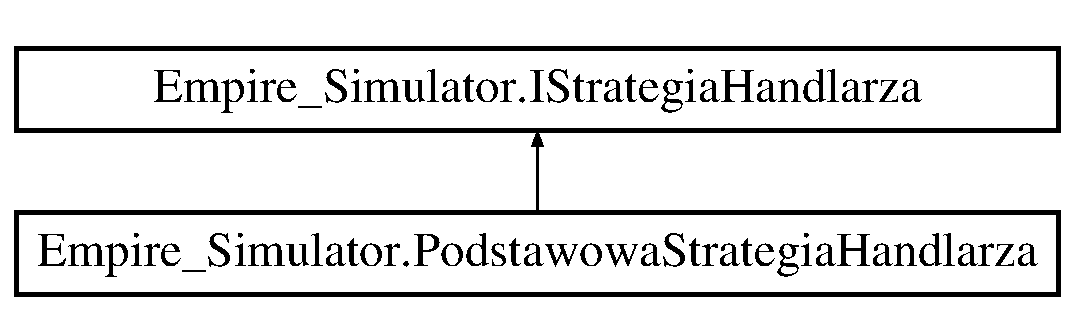
\includegraphics[height=2.000000cm]{interface_empire___simulator_1_1_i_strategia_handlarza}
\end{center}
\end{figure}
\subsection*{Public Member Functions}
\begin{DoxyCompactItemize}
\item 
\hypertarget{interface_empire___simulator_1_1_i_strategia_handlarza_af25c83bc6cd7cd012f16d15f5a5afe40}{\hyperlink{class_empire___simulator_1_1_osada}{Osada} {\bfseries wyznacz\+Cel\+Podrozy} (\hyperlink{class_empire___simulator_1_1_handlarz}{Handlarz} handlarz)}\label{interface_empire___simulator_1_1_i_strategia_handlarza_af25c83bc6cd7cd012f16d15f5a5afe40}

\item 
\hypertarget{interface_empire___simulator_1_1_i_strategia_handlarza_a6e2c9e3d418438ccb4e4aca310b3bc45}{Point {\bfseries podrozuj} (Point pozycja, Point cel\+Podrozy)}\label{interface_empire___simulator_1_1_i_strategia_handlarza_a6e2c9e3d418438ccb4e4aca310b3bc45}

\end{DoxyCompactItemize}


\subsection{Detailed Description}
Interfejs mówiący o tym jak wyznaczać nowy cel podróży dla handlarza oraz w jaki sposob sie przemieszcza 



The documentation for this interface was generated from the following file\+:\begin{DoxyCompactItemize}
\item 
C\+:/\+Users/\+Paweł/\+Documents/\+Git\+Hub/\+Empire\+\_\+\+Simulator\+\_\+\+V\+S\+\_\+2008/\+Empire\+\_\+\+Simulator/\+Empire\+\_\+\+Simulator/\+Interfejsy/I\+Strategia\+Handlarza.\+cs\end{DoxyCompactItemize}

\hypertarget{interface_empire___simulator_1_1_i_strategia_handlu}{\section{Empire\+\_\+\+Simulator.\+I\+Strategia\+Handlu Interface Reference}
\label{interface_empire___simulator_1_1_i_strategia_handlu}\index{Empire\+\_\+\+Simulator.\+I\+Strategia\+Handlu@{Empire\+\_\+\+Simulator.\+I\+Strategia\+Handlu}}
}


interfejs opisujacy jak wyglada wymiana towaru miedzy targiem a handlarzem  


Inheritance diagram for Empire\+\_\+\+Simulator.\+I\+Strategia\+Handlu\+:\begin{figure}[H]
\begin{center}
\leavevmode
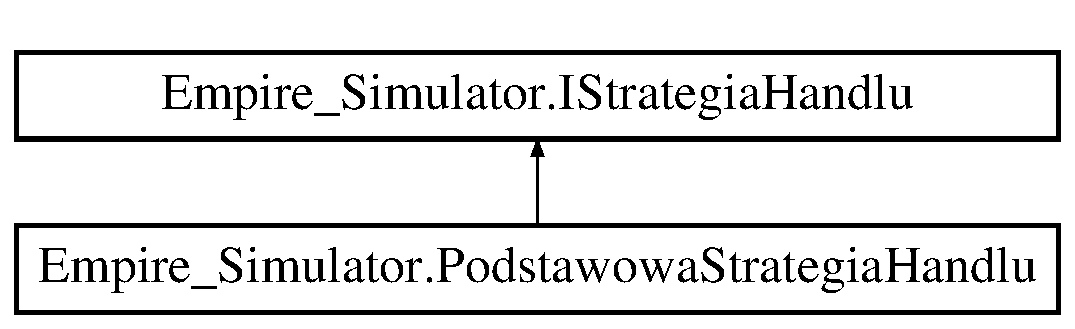
\includegraphics[height=2.000000cm]{interface_empire___simulator_1_1_i_strategia_handlu}
\end{center}
\end{figure}
\subsection*{Public Member Functions}
\begin{DoxyCompactItemize}
\item 
\hypertarget{interface_empire___simulator_1_1_i_strategia_handlu_a100f40aae9533b6f4301c3a839fe28c6}{void {\bfseries wymiana\+Towaru} (\hyperlink{class_empire___simulator_1_1_magazyn}{Magazyn} magazyn, \hyperlink{class_empire___simulator_1_1_handlarz}{Handlarz} handlarz, List$<$ string $>$ co\+Sprzedawac)}\label{interface_empire___simulator_1_1_i_strategia_handlu_a100f40aae9533b6f4301c3a839fe28c6}

\end{DoxyCompactItemize}


\subsection{Detailed Description}
interfejs opisujacy jak wyglada wymiana towaru miedzy targiem a handlarzem 



The documentation for this interface was generated from the following file\+:\begin{DoxyCompactItemize}
\item 
C\+:/\+Users/\+Paweł/\+Documents/\+Git\+Hub/\+Empire\+\_\+\+Simulator\+\_\+\+V\+S\+\_\+2008/\+Empire\+\_\+\+Simulator/\+Empire\+\_\+\+Simulator/\+Interfejsy/I\+Strategia\+Handlu.\+cs\end{DoxyCompactItemize}

\hypertarget{interface_empire___simulator_1_1_i_strategia_osady}{\section{Empire\+\_\+\+Simulator.\+I\+Strategia\+Osady Interface Reference}
\label{interface_empire___simulator_1_1_i_strategia_osady}\index{Empire\+\_\+\+Simulator.\+I\+Strategia\+Osady@{Empire\+\_\+\+Simulator.\+I\+Strategia\+Osady}}
}


Interfejs strategi osady wymusza metody których używa osada do zaktualizowania swojego statusu tj. stanow magazynowych i populacji, strategie bedą wymienne  


Inheritance diagram for Empire\+\_\+\+Simulator.\+I\+Strategia\+Osady\+:\begin{figure}[H]
\begin{center}
\leavevmode
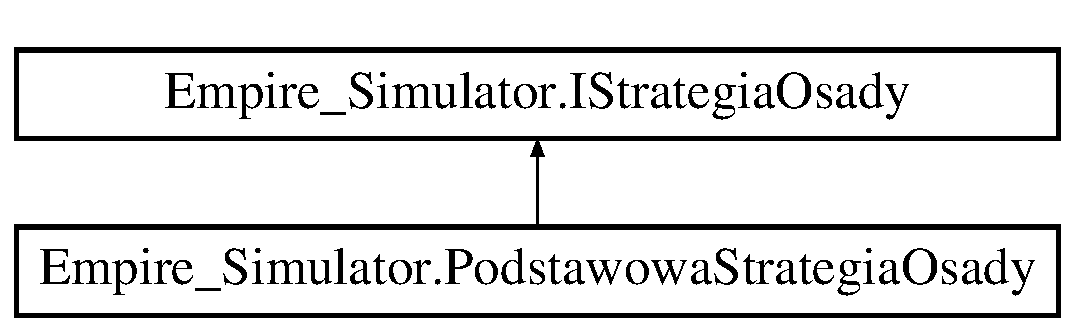
\includegraphics[height=2.000000cm]{interface_empire___simulator_1_1_i_strategia_osady}
\end{center}
\end{figure}
\subsection*{Public Member Functions}
\begin{DoxyCompactItemize}
\item 
void \hyperlink{interface_empire___simulator_1_1_i_strategia_osady_ac9ee9a6f745e76c2869f7561dfce9dd5}{aktualizuj\+Stan\+Populacji} (\hyperlink{class_empire___simulator_1_1_populacja}{Populacja} populacja, \hyperlink{class_empire___simulator_1_1_magazyn}{Magazyn} stan\+Magazynowy)
\begin{DoxyCompactList}\small\item\em Aktualizacja statnu popoulacji polega na zwiekszeniu lub zmiejszeniu populacji w zaleznosci od konkretnej strategi \end{DoxyCompactList}\item 
void \hyperlink{interface_empire___simulator_1_1_i_strategia_osady_a79abecf2ba585fb74915ed89fd7b06d6}{aktualizuj\+Stany\+Magazynowe} (\hyperlink{class_empire___simulator_1_1_magazyn}{Magazyn} magazyn, \hyperlink{class_empire___simulator_1_1_potencjal_wydobywczy}{Potencjal\+Wydobywczy} potencjal\+Wydobywczy, int liczba\+Ludnosci)
\begin{DoxyCompactList}\small\item\em aktualizacja stanów magazynowych polega na zwikszeniu lub zmiejszeniu stanow magazynowych w zależnosci od potencjalu wydobywczego itp. \end{DoxyCompactList}\end{DoxyCompactItemize}


\subsection{Detailed Description}
Interfejs strategi osady wymusza metody których używa osada do zaktualizowania swojego statusu tj. stanow magazynowych i populacji, strategie bedą wymienne 



\subsection{Member Function Documentation}
\hypertarget{interface_empire___simulator_1_1_i_strategia_osady_ac9ee9a6f745e76c2869f7561dfce9dd5}{\index{Empire\+\_\+\+Simulator\+::\+I\+Strategia\+Osady@{Empire\+\_\+\+Simulator\+::\+I\+Strategia\+Osady}!aktualizuj\+Stan\+Populacji@{aktualizuj\+Stan\+Populacji}}
\index{aktualizuj\+Stan\+Populacji@{aktualizuj\+Stan\+Populacji}!Empire\+\_\+\+Simulator\+::\+I\+Strategia\+Osady@{Empire\+\_\+\+Simulator\+::\+I\+Strategia\+Osady}}
\subsubsection[{aktualizuj\+Stan\+Populacji}]{\setlength{\rightskip}{0pt plus 5cm}void Empire\+\_\+\+Simulator.\+I\+Strategia\+Osady.\+aktualizuj\+Stan\+Populacji (
\begin{DoxyParamCaption}
\item[{{\bf Populacja}}]{populacja, }
\item[{{\bf Magazyn}}]{stan\+Magazynowy}
\end{DoxyParamCaption}
)}}\label{interface_empire___simulator_1_1_i_strategia_osady_ac9ee9a6f745e76c2869f7561dfce9dd5}


Aktualizacja statnu popoulacji polega na zwiekszeniu lub zmiejszeniu populacji w zaleznosci od konkretnej strategi 


\begin{DoxyParams}{Parameters}
{\em populacja} & \\
\hline
{\em stan\+Magazynowy} & \\
\hline
\end{DoxyParams}


Implemented in \hyperlink{class_empire___simulator_1_1_podstawowa_strategia_osady_a44cd6153770830086b7616b657d90e4e}{Empire\+\_\+\+Simulator.\+Podstawowa\+Strategia\+Osady}.

\hypertarget{interface_empire___simulator_1_1_i_strategia_osady_a79abecf2ba585fb74915ed89fd7b06d6}{\index{Empire\+\_\+\+Simulator\+::\+I\+Strategia\+Osady@{Empire\+\_\+\+Simulator\+::\+I\+Strategia\+Osady}!aktualizuj\+Stany\+Magazynowe@{aktualizuj\+Stany\+Magazynowe}}
\index{aktualizuj\+Stany\+Magazynowe@{aktualizuj\+Stany\+Magazynowe}!Empire\+\_\+\+Simulator\+::\+I\+Strategia\+Osady@{Empire\+\_\+\+Simulator\+::\+I\+Strategia\+Osady}}
\subsubsection[{aktualizuj\+Stany\+Magazynowe}]{\setlength{\rightskip}{0pt plus 5cm}void Empire\+\_\+\+Simulator.\+I\+Strategia\+Osady.\+aktualizuj\+Stany\+Magazynowe (
\begin{DoxyParamCaption}
\item[{{\bf Magazyn}}]{magazyn, }
\item[{{\bf Potencjal\+Wydobywczy}}]{potencjal\+Wydobywczy, }
\item[{int}]{liczba\+Ludnosci}
\end{DoxyParamCaption}
)}}\label{interface_empire___simulator_1_1_i_strategia_osady_a79abecf2ba585fb74915ed89fd7b06d6}


aktualizacja stanów magazynowych polega na zwikszeniu lub zmiejszeniu stanow magazynowych w zależnosci od potencjalu wydobywczego itp. 


\begin{DoxyParams}{Parameters}
{\em magazyn} & \\
\hline
{\em potencjal\+Wydobywczy} & \\
\hline
{\em liczba\+Ludnosci} & \\
\hline
\end{DoxyParams}


Implemented in \hyperlink{class_empire___simulator_1_1_podstawowa_strategia_osady_acf471696a52414814bd0608005c9518d}{Empire\+\_\+\+Simulator.\+Podstawowa\+Strategia\+Osady}.



The documentation for this interface was generated from the following file\+:\begin{DoxyCompactItemize}
\item 
C\+:/\+Users/\+Paweł/\+Documents/\+Git\+Hub/\+Empire\+\_\+\+Simulator\+\_\+\+V\+S\+\_\+2008/\+Empire\+\_\+\+Simulator/\+Empire\+\_\+\+Simulator/\+Interfejsy/I\+Strategia\+Osady.\+cs\end{DoxyCompactItemize}

\hypertarget{class_empire___simulator_1_1_losowanie_potencjalu}{\section{Empire\+\_\+\+Simulator.\+Losowanie\+Potencjalu Class Reference}
\label{class_empire___simulator_1_1_losowanie_potencjalu}\index{Empire\+\_\+\+Simulator.\+Losowanie\+Potencjalu@{Empire\+\_\+\+Simulator.\+Losowanie\+Potencjalu}}
}


zwraca liste wylosowanych zasobow.  


\subsection*{Public Member Functions}
\begin{DoxyCompactItemize}
\item 
\hypertarget{class_empire___simulator_1_1_losowanie_potencjalu_aeb24073a8ce0e9f26910fc099c8a1614}{{\bfseries Losowanie\+Potencjalu} (List$<$ string $>$ lista\+Zasobow, int ile\+Losowac)}\label{class_empire___simulator_1_1_losowanie_potencjalu_aeb24073a8ce0e9f26910fc099c8a1614}

\item 
\hyperlink{class_empire___simulator_1_1_potencjal_wydobywczy}{Potencjal\+Wydobywczy} \hyperlink{class_empire___simulator_1_1_losowanie_potencjalu_a4be2856bb8626faddeebd1d691da1b42}{generuj\+Potencjal} ()
\begin{DoxyCompactList}\small\item\em generuje gotowy obiekt potencjalu zawierajacy liste wydobywanych surowcow \end{DoxyCompactList}\end{DoxyCompactItemize}


\subsection{Detailed Description}
zwraca liste wylosowanych zasobow. 



\subsection{Member Function Documentation}
\hypertarget{class_empire___simulator_1_1_losowanie_potencjalu_a4be2856bb8626faddeebd1d691da1b42}{\index{Empire\+\_\+\+Simulator\+::\+Losowanie\+Potencjalu@{Empire\+\_\+\+Simulator\+::\+Losowanie\+Potencjalu}!generuj\+Potencjal@{generuj\+Potencjal}}
\index{generuj\+Potencjal@{generuj\+Potencjal}!Empire\+\_\+\+Simulator\+::\+Losowanie\+Potencjalu@{Empire\+\_\+\+Simulator\+::\+Losowanie\+Potencjalu}}
\subsubsection[{generuj\+Potencjal}]{\setlength{\rightskip}{0pt plus 5cm}{\bf Potencjal\+Wydobywczy} Empire\+\_\+\+Simulator.\+Losowanie\+Potencjalu.\+generuj\+Potencjal (
\begin{DoxyParamCaption}
{}
\end{DoxyParamCaption}
)\hspace{0.3cm}{\ttfamily [inline]}}}\label{class_empire___simulator_1_1_losowanie_potencjalu_a4be2856bb8626faddeebd1d691da1b42}


generuje gotowy obiekt potencjalu zawierajacy liste wydobywanych surowcow 

\begin{DoxyReturn}{Returns}
obiekt potencjału
\end{DoxyReturn}


The documentation for this class was generated from the following file\+:\begin{DoxyCompactItemize}
\item 
C\+:/\+Users/\+Paweł/\+Documents/\+Git\+Hub/\+Empire\+\_\+\+Simulator\+\_\+\+V\+S\+\_\+2008/\+Empire\+\_\+\+Simulator/\+Empire\+\_\+\+Simulator/\+Klasy/\+Zasob/Losowanie\+Potencjalu.\+cs\end{DoxyCompactItemize}

\hypertarget{class_empire___simulator_1_1_losowanie_zasobu}{\section{Empire\+\_\+\+Simulator.\+Losowanie\+Zasobu Class Reference}
\label{class_empire___simulator_1_1_losowanie_zasobu}\index{Empire\+\_\+\+Simulator.\+Losowanie\+Zasobu@{Empire\+\_\+\+Simulator.\+Losowanie\+Zasobu}}
}


Tworzy obiekt potrafiacy wylosowac liczbe z zadanego mu przedzialu  


\subsection*{Public Member Functions}
\begin{DoxyCompactItemize}
\item 
\hypertarget{class_empire___simulator_1_1_losowanie_zasobu_aaebf0e1c3819eefae2a01c36c7bdd480}{{\bfseries Losowanie\+Zasobu} (int minimum, int maksimum)}\label{class_empire___simulator_1_1_losowanie_zasobu_aaebf0e1c3819eefae2a01c36c7bdd480}

\item 
int \hyperlink{class_empire___simulator_1_1_losowanie_zasobu_afd8b2d6873100e8e4ffed05e8e837a62}{losuj\+Zasob} ()
\begin{DoxyCompactList}\small\item\em zraca wartosc int ktora bedzie z przedzialu minimum a maksimum jakos ze losujemy od zera do maksimum to do wylosowanej liczby dodajemy minimum dzieki czemu najnizsza wartosc jaka dostaniemy jest wlasnie minimum w przypadku gdy generator losuje zero \end{DoxyCompactList}\end{DoxyCompactItemize}


\subsection{Detailed Description}
Tworzy obiekt potrafiacy wylosowac liczbe z zadanego mu przedzialu 



\subsection{Member Function Documentation}
\hypertarget{class_empire___simulator_1_1_losowanie_zasobu_afd8b2d6873100e8e4ffed05e8e837a62}{\index{Empire\+\_\+\+Simulator\+::\+Losowanie\+Zasobu@{Empire\+\_\+\+Simulator\+::\+Losowanie\+Zasobu}!losuj\+Zasob@{losuj\+Zasob}}
\index{losuj\+Zasob@{losuj\+Zasob}!Empire\+\_\+\+Simulator\+::\+Losowanie\+Zasobu@{Empire\+\_\+\+Simulator\+::\+Losowanie\+Zasobu}}
\subsubsection[{losuj\+Zasob}]{\setlength{\rightskip}{0pt plus 5cm}int Empire\+\_\+\+Simulator.\+Losowanie\+Zasobu.\+losuj\+Zasob (
\begin{DoxyParamCaption}
{}
\end{DoxyParamCaption}
)\hspace{0.3cm}{\ttfamily [inline]}}}\label{class_empire___simulator_1_1_losowanie_zasobu_afd8b2d6873100e8e4ffed05e8e837a62}


zraca wartosc int ktora bedzie z przedzialu minimum a maksimum jakos ze losujemy od zera do maksimum to do wylosowanej liczby dodajemy minimum dzieki czemu najnizsza wartosc jaka dostaniemy jest wlasnie minimum w przypadku gdy generator losuje zero 

\begin{DoxyReturn}{Returns}

\end{DoxyReturn}


The documentation for this class was generated from the following file\+:\begin{DoxyCompactItemize}
\item 
C\+:/\+Users/\+Paweł/\+Documents/\+Git\+Hub/\+Empire\+\_\+\+Simulator\+\_\+\+V\+S\+\_\+2008/\+Empire\+\_\+\+Simulator/\+Empire\+\_\+\+Simulator/\+Klasy/\+Zasob/Losowanie\+Zasobu.\+cs\end{DoxyCompactItemize}

\hypertarget{class_empire___simulator_1_1_magazyn}{\section{Empire\+\_\+\+Simulator.\+Magazyn Class Reference}
\label{class_empire___simulator_1_1_magazyn}\index{Empire\+\_\+\+Simulator.\+Magazyn@{Empire\+\_\+\+Simulator.\+Magazyn}}
}


\hyperlink{class_empire___simulator_1_1_magazyn}{Magazyn} jest obiektem posiadanym przez osadę, i przetrzymującym w swoich polach ilośći zasobów posiadane przez ową wioskę  


\subsection*{Public Member Functions}
\begin{DoxyCompactItemize}
\item 
\hypertarget{class_empire___simulator_1_1_magazyn_aa4e695b9b8d8bda4fa76e4d628688335}{{\bfseries Magazyn} (Dictionary$<$ string, \hyperlink{class_empire___simulator_1_1_zasob}{Zasob} $>$ zasoby)}\label{class_empire___simulator_1_1_magazyn_aa4e695b9b8d8bda4fa76e4d628688335}

\item 
Dictionary$<$ string, \hyperlink{class_empire___simulator_1_1_zasob}{Zasob} $>$ \hyperlink{class_empire___simulator_1_1_magazyn_aa9eb4e63d4b3d495af6d9b2f40ea2cd3}{pobierz\+Stan\+Magazynu} ()
\begin{DoxyCompactList}\small\item\em metoda zwracająca obecny stan Magazynu \end{DoxyCompactList}\item 
\hypertarget{class_empire___simulator_1_1_magazyn_a2e194935669e0531b6b7e1e746d0f828}{override string {\bfseries To\+String} ()}\label{class_empire___simulator_1_1_magazyn_a2e194935669e0531b6b7e1e746d0f828}

\end{DoxyCompactItemize}


\subsection{Detailed Description}
\hyperlink{class_empire___simulator_1_1_magazyn}{Magazyn} jest obiektem posiadanym przez osadę, i przetrzymującym w swoich polach ilośći zasobów posiadane przez ową wioskę 



\subsection{Member Function Documentation}
\hypertarget{class_empire___simulator_1_1_magazyn_aa9eb4e63d4b3d495af6d9b2f40ea2cd3}{\index{Empire\+\_\+\+Simulator\+::\+Magazyn@{Empire\+\_\+\+Simulator\+::\+Magazyn}!pobierz\+Stan\+Magazynu@{pobierz\+Stan\+Magazynu}}
\index{pobierz\+Stan\+Magazynu@{pobierz\+Stan\+Magazynu}!Empire\+\_\+\+Simulator\+::\+Magazyn@{Empire\+\_\+\+Simulator\+::\+Magazyn}}
\subsubsection[{pobierz\+Stan\+Magazynu}]{\setlength{\rightskip}{0pt plus 5cm}Dictionary$<$string, {\bf Zasob}$>$ Empire\+\_\+\+Simulator.\+Magazyn.\+pobierz\+Stan\+Magazynu (
\begin{DoxyParamCaption}
{}
\end{DoxyParamCaption}
)\hspace{0.3cm}{\ttfamily [inline]}}}\label{class_empire___simulator_1_1_magazyn_aa9eb4e63d4b3d495af6d9b2f40ea2cd3}


metoda zwracająca obecny stan Magazynu 

\begin{DoxyReturn}{Returns}
słownik zawierajacy stan magazynu
\end{DoxyReturn}


The documentation for this class was generated from the following file\+:\begin{DoxyCompactItemize}
\item 
C\+:/\+Users/\+Paweł/\+Documents/\+Git\+Hub/\+Empire\+\_\+\+Simulator\+\_\+\+V\+S\+\_\+2008/\+Empire\+\_\+\+Simulator/\+Empire\+\_\+\+Simulator/\+Klasy/\+Osada/Magazyn.\+cs\end{DoxyCompactItemize}

\hypertarget{class_empire___simulator_1_1_okno_gry}{\section{Empire\+\_\+\+Simulator.\+Okno\+Gry Class Reference}
\label{class_empire___simulator_1_1_okno_gry}\index{Empire\+\_\+\+Simulator.\+Okno\+Gry@{Empire\+\_\+\+Simulator.\+Okno\+Gry}}
}


Jest to główne okno gry  


Inheritance diagram for Empire\+\_\+\+Simulator.\+Okno\+Gry\+:\begin{figure}[H]
\begin{center}
\leavevmode
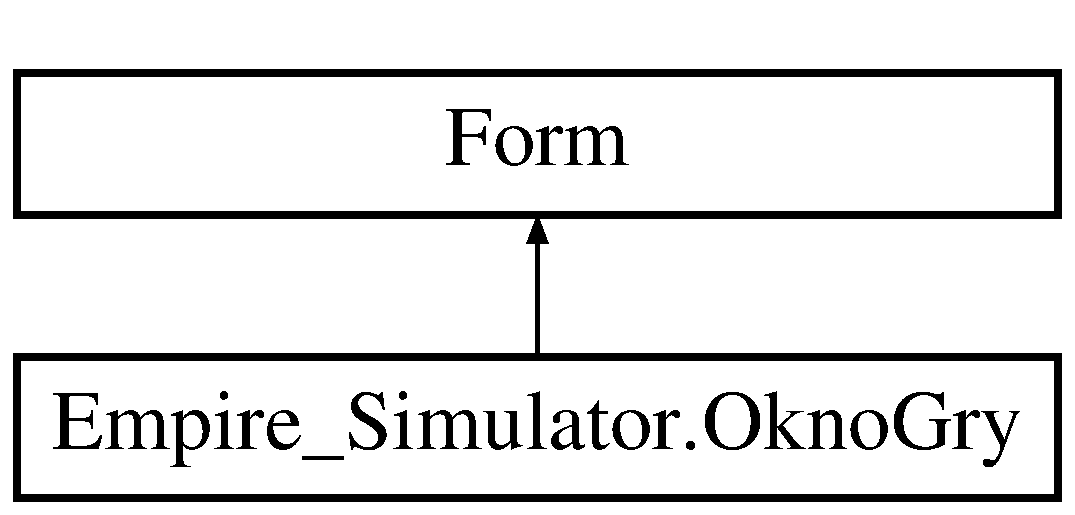
\includegraphics[height=2.000000cm]{class_empire___simulator_1_1_okno_gry}
\end{center}
\end{figure}
\subsection*{Public Member Functions}
\begin{DoxyCompactItemize}
\item 
\hypertarget{class_empire___simulator_1_1_okno_gry_a7aa35cd006097d16c37de5ad5be7e8cd}{{\bfseries Okno\+Gry} (\hyperlink{class_empire___simulator_1_1_swiat}{Swiat} swiat)}\label{class_empire___simulator_1_1_okno_gry_a7aa35cd006097d16c37de5ad5be7e8cd}

\end{DoxyCompactItemize}
\subsection*{Protected Member Functions}
\begin{DoxyCompactItemize}
\item 
override void \hyperlink{class_empire___simulator_1_1_okno_gry_aa5626b7864ef1f2465646b0305b10431}{Dispose} (bool disposing)
\begin{DoxyCompactList}\small\item\em Clean up any resources being used. \end{DoxyCompactList}\end{DoxyCompactItemize}


\subsection{Detailed Description}
Jest to główne okno gry 



\subsection{Member Function Documentation}
\hypertarget{class_empire___simulator_1_1_okno_gry_aa5626b7864ef1f2465646b0305b10431}{\index{Empire\+\_\+\+Simulator\+::\+Okno\+Gry@{Empire\+\_\+\+Simulator\+::\+Okno\+Gry}!Dispose@{Dispose}}
\index{Dispose@{Dispose}!Empire\+\_\+\+Simulator\+::\+Okno\+Gry@{Empire\+\_\+\+Simulator\+::\+Okno\+Gry}}
\subsubsection[{Dispose}]{\setlength{\rightskip}{0pt plus 5cm}override void Empire\+\_\+\+Simulator.\+Okno\+Gry.\+Dispose (
\begin{DoxyParamCaption}
\item[{bool}]{disposing}
\end{DoxyParamCaption}
)\hspace{0.3cm}{\ttfamily [inline]}, {\ttfamily [protected]}}}\label{class_empire___simulator_1_1_okno_gry_aa5626b7864ef1f2465646b0305b10431}


Clean up any resources being used. 


\begin{DoxyParams}{Parameters}
{\em disposing} & true if managed resources should be disposed; otherwise, false.\\
\hline
\end{DoxyParams}


The documentation for this class was generated from the following files\+:\begin{DoxyCompactItemize}
\item 
C\+:/\+Users/\+Paweł/\+Documents/\+Git\+Hub/\+Empire\+\_\+\+Simulator\+\_\+\+V\+S\+\_\+2008/\+Empire\+\_\+\+Simulator/\+Empire\+\_\+\+Simulator/\+Mapa/Okno\+Gry.\+cs\item 
C\+:/\+Users/\+Paweł/\+Documents/\+Git\+Hub/\+Empire\+\_\+\+Simulator\+\_\+\+V\+S\+\_\+2008/\+Empire\+\_\+\+Simulator/\+Empire\+\_\+\+Simulator/\+Mapa/Okno\+Gry.\+Designer.\+cs\end{DoxyCompactItemize}

\hypertarget{class_empire___simulator_1_1_osada}{\section{Empire\+\_\+\+Simulator.\+Osada Class Reference}
\label{class_empire___simulator_1_1_osada}\index{Empire\+\_\+\+Simulator.\+Osada@{Empire\+\_\+\+Simulator.\+Osada}}
}


Klasa Tworzaca obiekt osady  


\subsection*{Public Member Functions}
\begin{DoxyCompactItemize}
\item 
\hypertarget{class_empire___simulator_1_1_osada_ab1adf9544300c191346c100fb52e65b2}{{\bfseries Osada} (\hyperlink{interface_empire___simulator_1_1_i_strategia_osady}{I\+Strategia\+Osady} strategia, \hyperlink{interface_empire___simulator_1_1_i_strategia_handlu}{I\+Strategia\+Handlu} strategia\+Handlu, string nazwa, \hyperlink{class_empire___simulator_1_1_magazyn}{Magazyn} magazyn, \hyperlink{class_empire___simulator_1_1_populacja}{Populacja} populacja, \hyperlink{class_empire___simulator_1_1_potencjal_wydobywczy}{Potencjal\+Wydobywczy} potencjal\+Wydobywczy, Point pozycja)}\label{class_empire___simulator_1_1_osada_ab1adf9544300c191346c100fb52e65b2}

\item 
\hyperlink{class_empire___simulator_1_1_targ}{Targ} \hyperlink{class_empire___simulator_1_1_osada_a57b436a278a3003b0acbd1adf0bb425e}{Targowisko} ()
\begin{DoxyCompactList}\small\item\em zwraca \hyperlink{class_empire___simulator_1_1_targ}{Targ} \end{DoxyCompactList}\item 
void \hyperlink{class_empire___simulator_1_1_osada_a9c261a758d377f2a49fb1acd18df71ae}{aktualizuj} ()
\begin{DoxyCompactList}\small\item\em Aktualizujue swój stan tj magazyny i populacje, korzystając ze strategi \end{DoxyCompactList}\item 
\hyperlink{class_empire___simulator_1_1_magazyn}{Magazyn} \hyperlink{class_empire___simulator_1_1_osada_a781412cccc2c86c3ac33ad32384a40ee}{magazyny} ()
\begin{DoxyCompactList}\small\item\em Zwraca magazyn zastanawiam sie czy to nie jest tylko metoda testowa. \end{DoxyCompactList}\item 
\hypertarget{class_empire___simulator_1_1_osada_a3221155c2b3d083f01e6f4f2f0f2815c}{Point {\bfseries pozycja\+Osady} ()}\label{class_empire___simulator_1_1_osada_a3221155c2b3d083f01e6f4f2f0f2815c}

\item 
\hypertarget{class_empire___simulator_1_1_osada_af2c60f054a22039a7dcfc7b895c89a88}{int {\bfseries populacja\+Osady} ()}\label{class_empire___simulator_1_1_osada_af2c60f054a22039a7dcfc7b895c89a88}

\item 
\hypertarget{class_empire___simulator_1_1_osada_a14a436bd6345e7feb0c845eb28ce7223}{override string {\bfseries To\+String} ()}\label{class_empire___simulator_1_1_osada_a14a436bd6345e7feb0c845eb28ce7223}

\end{DoxyCompactItemize}


\subsection{Detailed Description}
Klasa Tworzaca obiekt osady 



\subsection{Member Function Documentation}
\hypertarget{class_empire___simulator_1_1_osada_a9c261a758d377f2a49fb1acd18df71ae}{\index{Empire\+\_\+\+Simulator\+::\+Osada@{Empire\+\_\+\+Simulator\+::\+Osada}!aktualizuj@{aktualizuj}}
\index{aktualizuj@{aktualizuj}!Empire\+\_\+\+Simulator\+::\+Osada@{Empire\+\_\+\+Simulator\+::\+Osada}}
\subsubsection[{aktualizuj}]{\setlength{\rightskip}{0pt plus 5cm}void Empire\+\_\+\+Simulator.\+Osada.\+aktualizuj (
\begin{DoxyParamCaption}
{}
\end{DoxyParamCaption}
)\hspace{0.3cm}{\ttfamily [inline]}}}\label{class_empire___simulator_1_1_osada_a9c261a758d377f2a49fb1acd18df71ae}


Aktualizujue swój stan tj magazyny i populacje, korzystając ze strategi 

\hypertarget{class_empire___simulator_1_1_osada_a781412cccc2c86c3ac33ad32384a40ee}{\index{Empire\+\_\+\+Simulator\+::\+Osada@{Empire\+\_\+\+Simulator\+::\+Osada}!magazyny@{magazyny}}
\index{magazyny@{magazyny}!Empire\+\_\+\+Simulator\+::\+Osada@{Empire\+\_\+\+Simulator\+::\+Osada}}
\subsubsection[{magazyny}]{\setlength{\rightskip}{0pt plus 5cm}{\bf Magazyn} Empire\+\_\+\+Simulator.\+Osada.\+magazyny (
\begin{DoxyParamCaption}
{}
\end{DoxyParamCaption}
)\hspace{0.3cm}{\ttfamily [inline]}}}\label{class_empire___simulator_1_1_osada_a781412cccc2c86c3ac33ad32384a40ee}


Zwraca magazyn zastanawiam sie czy to nie jest tylko metoda testowa. 

\begin{DoxyReturn}{Returns}

\end{DoxyReturn}
\hypertarget{class_empire___simulator_1_1_osada_a57b436a278a3003b0acbd1adf0bb425e}{\index{Empire\+\_\+\+Simulator\+::\+Osada@{Empire\+\_\+\+Simulator\+::\+Osada}!Targowisko@{Targowisko}}
\index{Targowisko@{Targowisko}!Empire\+\_\+\+Simulator\+::\+Osada@{Empire\+\_\+\+Simulator\+::\+Osada}}
\subsubsection[{Targowisko}]{\setlength{\rightskip}{0pt plus 5cm}{\bf Targ} Empire\+\_\+\+Simulator.\+Osada.\+Targowisko (
\begin{DoxyParamCaption}
{}
\end{DoxyParamCaption}
)\hspace{0.3cm}{\ttfamily [inline]}}}\label{class_empire___simulator_1_1_osada_a57b436a278a3003b0acbd1adf0bb425e}


zwraca \hyperlink{class_empire___simulator_1_1_targ}{Targ} 

\begin{DoxyReturn}{Returns}
obiekt \hyperlink{class_empire___simulator_1_1_targ}{Targ}
\end{DoxyReturn}


The documentation for this class was generated from the following file\+:\begin{DoxyCompactItemize}
\item 
C\+:/\+Users/\+Paweł/\+Documents/\+Git\+Hub/\+Empire\+\_\+\+Simulator\+\_\+\+V\+S\+\_\+2008/\+Empire\+\_\+\+Simulator/\+Empire\+\_\+\+Simulator/\+Klasy/\+Osada/Osada.\+cs\end{DoxyCompactItemize}

\hypertarget{class_empire___simulator_1_1_podstawowa_strategia_aktualizacji_swiata}{\section{Empire\+\_\+\+Simulator.\+Podstawowa\+Strategia\+Aktualizacji\+Swiata Class Reference}
\label{class_empire___simulator_1_1_podstawowa_strategia_aktualizacji_swiata}\index{Empire\+\_\+\+Simulator.\+Podstawowa\+Strategia\+Aktualizacji\+Swiata@{Empire\+\_\+\+Simulator.\+Podstawowa\+Strategia\+Aktualizacji\+Swiata}}
}
Inheritance diagram for Empire\+\_\+\+Simulator.\+Podstawowa\+Strategia\+Aktualizacji\+Swiata\+:\begin{figure}[H]
\begin{center}
\leavevmode
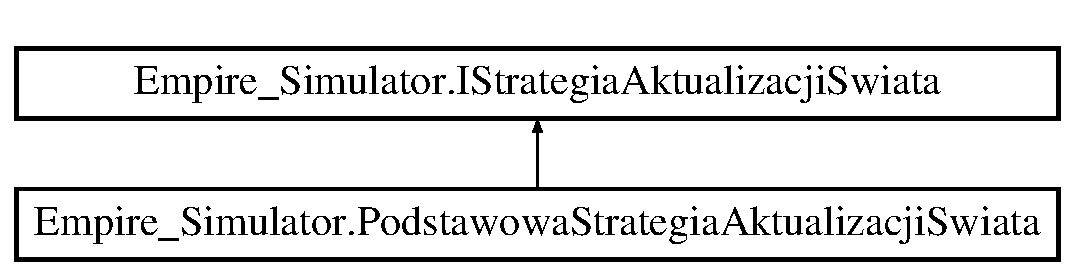
\includegraphics[height=2.000000cm]{class_empire___simulator_1_1_podstawowa_strategia_aktualizacji_swiata}
\end{center}
\end{figure}
\subsection*{Public Member Functions}
\begin{DoxyCompactItemize}
\item 
\hypertarget{class_empire___simulator_1_1_podstawowa_strategia_aktualizacji_swiata_a09269ca116583011493af41a63bf09c7}{int {\bfseries co\+Ile\+Dni\+Aktualizowac\+Osade} ()}\label{class_empire___simulator_1_1_podstawowa_strategia_aktualizacji_swiata_a09269ca116583011493af41a63bf09c7}

\item 
\hypertarget{class_empire___simulator_1_1_podstawowa_strategia_aktualizacji_swiata_a961720f39c96c8f938daf174eb395c02}{int {\bfseries co\+Ile\+Dni\+Aktualizowac\+Handlarza} ()}\label{class_empire___simulator_1_1_podstawowa_strategia_aktualizacji_swiata_a961720f39c96c8f938daf174eb395c02}

\end{DoxyCompactItemize}


The documentation for this class was generated from the following file\+:\begin{DoxyCompactItemize}
\item 
C\+:/\+Users/\+Paweł/\+Documents/\+Git\+Hub/\+Empire\+\_\+\+Simulator\+\_\+\+V\+S\+\_\+2008/\+Empire\+\_\+\+Simulator/\+Empire\+\_\+\+Simulator/\+Strategie/Podstawowa\+Strategia\+Aktualizacji\+Swiata.\+cs\end{DoxyCompactItemize}

\hypertarget{class_empire___simulator_1_1_podstawowa_strategia_generowania_swiata}{\section{Empire\+\_\+\+Simulator.\+Podstawowa\+Strategia\+Generowania\+Swiata Class Reference}
\label{class_empire___simulator_1_1_podstawowa_strategia_generowania_swiata}\index{Empire\+\_\+\+Simulator.\+Podstawowa\+Strategia\+Generowania\+Swiata@{Empire\+\_\+\+Simulator.\+Podstawowa\+Strategia\+Generowania\+Swiata}}
}
Inheritance diagram for Empire\+\_\+\+Simulator.\+Podstawowa\+Strategia\+Generowania\+Swiata\+:\begin{figure}[H]
\begin{center}
\leavevmode
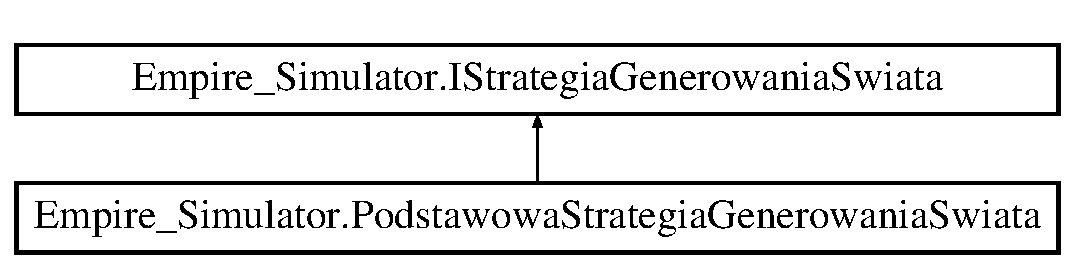
\includegraphics[height=2.000000cm]{class_empire___simulator_1_1_podstawowa_strategia_generowania_swiata}
\end{center}
\end{figure}
\subsection*{Public Member Functions}
\begin{DoxyCompactItemize}
\item 
\hypertarget{class_empire___simulator_1_1_podstawowa_strategia_generowania_swiata_ae20cc6da6e2488cc8f390345a990205b}{int {\bfseries ilosc\+Osad\+Do\+Wygenerowania} ()}\label{class_empire___simulator_1_1_podstawowa_strategia_generowania_swiata_ae20cc6da6e2488cc8f390345a990205b}

\item 
\hypertarget{class_empire___simulator_1_1_podstawowa_strategia_generowania_swiata_ad6fde99a86ea7e05a266fdbb26fa1a5a}{int {\bfseries ilosc\+Handlarzy\+Do\+Wygenerowania} ()}\label{class_empire___simulator_1_1_podstawowa_strategia_generowania_swiata_ad6fde99a86ea7e05a266fdbb26fa1a5a}

\item 
\hypertarget{class_empire___simulator_1_1_podstawowa_strategia_generowania_swiata_a0b8b25ecba4d2128ad665db882d04c9e}{int {\bfseries pojemnosc\+Wozu\+Handlarza} ()}\label{class_empire___simulator_1_1_podstawowa_strategia_generowania_swiata_a0b8b25ecba4d2128ad665db882d04c9e}

\item 
\hypertarget{class_empire___simulator_1_1_podstawowa_strategia_generowania_swiata_a24e2b1b4c6513295abfa1d1b806b6ad8}{\hyperlink{interface_empire___simulator_1_1_i_strategia_handlarza}{I\+Strategia\+Handlarza} {\bfseries strategia\+Handlarza} (List$<$ \hyperlink{class_empire___simulator_1_1_osada}{Osada} $>$lista\+Osad, List$<$ \hyperlink{class_empire___simulator_1_1_handlarz}{Handlarz} $>$ lista\+Handlarzy)}\label{class_empire___simulator_1_1_podstawowa_strategia_generowania_swiata_a24e2b1b4c6513295abfa1d1b806b6ad8}

\item 
\hypertarget{class_empire___simulator_1_1_podstawowa_strategia_generowania_swiata_a768550bd1c8b8363f9779d1a02e50286}{\hyperlink{interface_empire___simulator_1_1_i_strategia_handlu}{I\+Strategia\+Handlu} {\bfseries strategia\+Handlu} ()}\label{class_empire___simulator_1_1_podstawowa_strategia_generowania_swiata_a768550bd1c8b8363f9779d1a02e50286}

\item 
\hypertarget{class_empire___simulator_1_1_podstawowa_strategia_generowania_swiata_a0a2d7749efdcc7ccbb6143f28502a287}{\hyperlink{interface_empire___simulator_1_1_i_strategia_osady}{I\+Strategia\+Osady} {\bfseries strategia\+Osady} ()}\label{class_empire___simulator_1_1_podstawowa_strategia_generowania_swiata_a0a2d7749efdcc7ccbb6143f28502a287}

\end{DoxyCompactItemize}


The documentation for this class was generated from the following file\+:\begin{DoxyCompactItemize}
\item 
C\+:/\+Users/\+Paweł/\+Documents/\+Git\+Hub/\+Empire\+\_\+\+Simulator\+\_\+\+V\+S\+\_\+2008/\+Empire\+\_\+\+Simulator/\+Empire\+\_\+\+Simulator/\+Strategie/Podstawowa\+Strategia\+Generowania\+Swiata.\+cs\end{DoxyCompactItemize}

\hypertarget{class_empire___simulator_1_1_podstawowa_strategia_handlarza}{\section{Empire\+\_\+\+Simulator.\+Podstawowa\+Strategia\+Handlarza Class Reference}
\label{class_empire___simulator_1_1_podstawowa_strategia_handlarza}\index{Empire\+\_\+\+Simulator.\+Podstawowa\+Strategia\+Handlarza@{Empire\+\_\+\+Simulator.\+Podstawowa\+Strategia\+Handlarza}}
}
Inheritance diagram for Empire\+\_\+\+Simulator.\+Podstawowa\+Strategia\+Handlarza\+:\begin{figure}[H]
\begin{center}
\leavevmode
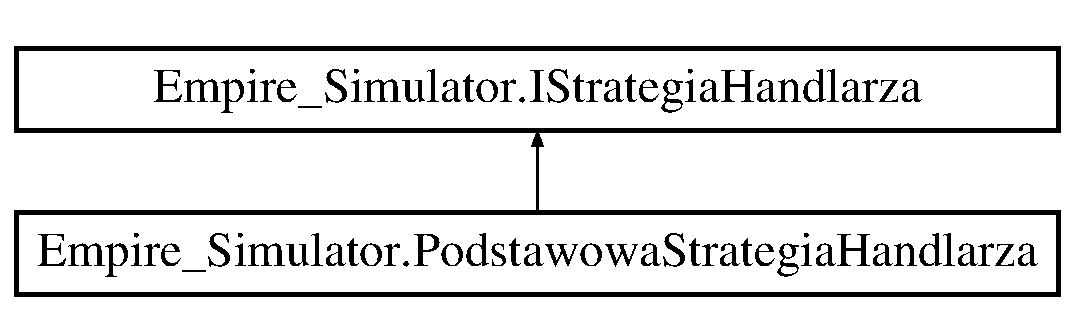
\includegraphics[height=2.000000cm]{class_empire___simulator_1_1_podstawowa_strategia_handlarza}
\end{center}
\end{figure}
\subsection*{Public Member Functions}
\begin{DoxyCompactItemize}
\item 
\hypertarget{class_empire___simulator_1_1_podstawowa_strategia_handlarza_a1a2f087d5b7b653da35e853f8b43b757}{{\bfseries Podstawowa\+Strategia\+Handlarza} (List$<$ \hyperlink{class_empire___simulator_1_1_osada}{Osada} $>$ lista\+Osad, List$<$ \hyperlink{class_empire___simulator_1_1_handlarz}{Handlarz} $>$ lista\+Handlarzy)}\label{class_empire___simulator_1_1_podstawowa_strategia_handlarza_a1a2f087d5b7b653da35e853f8b43b757}

\item 
\hyperlink{class_empire___simulator_1_1_osada}{Osada} \hyperlink{class_empire___simulator_1_1_podstawowa_strategia_handlarza_a6897f69ec6e2093883828eaddb1c5c5c}{wyznacz\+Cel\+Podrozy} (\hyperlink{class_empire___simulator_1_1_handlarz}{Handlarz} handlarz)
\begin{DoxyCompactList}\small\item\em Wyznaczanie celu podrozy poprzez wybranie wioski ktora ma najmniej surowca ktory posiada handlarz \end{DoxyCompactList}\item 
\hypertarget{class_empire___simulator_1_1_podstawowa_strategia_handlarza_a34abee39189969d506078f7ea96aefc2}{Point {\bfseries podrozuj} (Point pozycja, Point cel\+Podrozy)}\label{class_empire___simulator_1_1_podstawowa_strategia_handlarza_a34abee39189969d506078f7ea96aefc2}

\end{DoxyCompactItemize}


\subsection{Member Function Documentation}
\hypertarget{class_empire___simulator_1_1_podstawowa_strategia_handlarza_a6897f69ec6e2093883828eaddb1c5c5c}{\index{Empire\+\_\+\+Simulator\+::\+Podstawowa\+Strategia\+Handlarza@{Empire\+\_\+\+Simulator\+::\+Podstawowa\+Strategia\+Handlarza}!wyznacz\+Cel\+Podrozy@{wyznacz\+Cel\+Podrozy}}
\index{wyznacz\+Cel\+Podrozy@{wyznacz\+Cel\+Podrozy}!Empire\+\_\+\+Simulator\+::\+Podstawowa\+Strategia\+Handlarza@{Empire\+\_\+\+Simulator\+::\+Podstawowa\+Strategia\+Handlarza}}
\subsubsection[{wyznacz\+Cel\+Podrozy}]{\setlength{\rightskip}{0pt plus 5cm}{\bf Osada} Empire\+\_\+\+Simulator.\+Podstawowa\+Strategia\+Handlarza.\+wyznacz\+Cel\+Podrozy (
\begin{DoxyParamCaption}
\item[{{\bf Handlarz}}]{handlarz}
\end{DoxyParamCaption}
)\hspace{0.3cm}{\ttfamily [inline]}}}\label{class_empire___simulator_1_1_podstawowa_strategia_handlarza_a6897f69ec6e2093883828eaddb1c5c5c}


Wyznaczanie celu podrozy poprzez wybranie wioski ktora ma najmniej surowca ktory posiada handlarz 


\begin{DoxyParams}{Parameters}
{\em handlarz} & \\
\hline
\end{DoxyParams}
\begin{DoxyReturn}{Returns}

\end{DoxyReturn}


Implements \hyperlink{interface_empire___simulator_1_1_i_strategia_handlarza}{Empire\+\_\+\+Simulator.\+I\+Strategia\+Handlarza}.



The documentation for this class was generated from the following file\+:\begin{DoxyCompactItemize}
\item 
C\+:/\+Users/\+Paweł/\+Documents/\+Git\+Hub/\+Empire\+\_\+\+Simulator\+\_\+\+V\+S\+\_\+2008/\+Empire\+\_\+\+Simulator/\+Empire\+\_\+\+Simulator/\+Strategie/Podstawowa\+Strategia\+Handlarza.\+cs\end{DoxyCompactItemize}

\hypertarget{class_empire___simulator_1_1_podstawowa_strategia_handlu}{\section{Empire\+\_\+\+Simulator.\+Podstawowa\+Strategia\+Handlu Class Reference}
\label{class_empire___simulator_1_1_podstawowa_strategia_handlu}\index{Empire\+\_\+\+Simulator.\+Podstawowa\+Strategia\+Handlu@{Empire\+\_\+\+Simulator.\+Podstawowa\+Strategia\+Handlu}}
}
Inheritance diagram for Empire\+\_\+\+Simulator.\+Podstawowa\+Strategia\+Handlu\+:\begin{figure}[H]
\begin{center}
\leavevmode
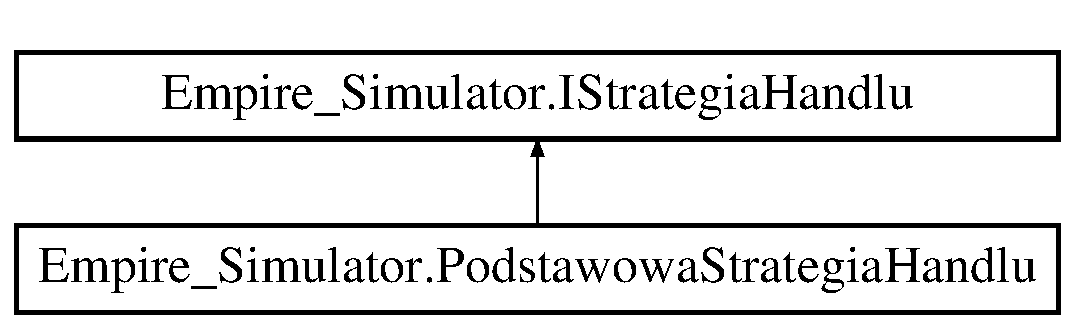
\includegraphics[height=2.000000cm]{class_empire___simulator_1_1_podstawowa_strategia_handlu}
\end{center}
\end{figure}
\subsection*{Public Member Functions}
\begin{DoxyCompactItemize}
\item 
void \hyperlink{class_empire___simulator_1_1_podstawowa_strategia_handlu_ae653aa636d479f2da21fa575320c56e9}{wymiana\+Towaru} (\hyperlink{class_empire___simulator_1_1_magazyn}{Magazyn} magazyn, \hyperlink{class_empire___simulator_1_1_handlarz}{Handlarz} handlarz, List$<$ string $>$ co\+Sprzedawac)
\begin{DoxyCompactList}\small\item\em Obecna wymiana polega na tym ze handlarz wymienia sie z targiem porowno, tj rozladowuje swoje zasoby i sa ladowane do magazynua potem z magazynu bierzemy surowiec ktorego jest najwiecej i ladujemy mu na woz Pożadana strategia jest raczej inna, pozniewaz obecna jest strasznie trywialna. \end{DoxyCompactList}\end{DoxyCompactItemize}


\subsection{Member Function Documentation}
\hypertarget{class_empire___simulator_1_1_podstawowa_strategia_handlu_ae653aa636d479f2da21fa575320c56e9}{\index{Empire\+\_\+\+Simulator\+::\+Podstawowa\+Strategia\+Handlu@{Empire\+\_\+\+Simulator\+::\+Podstawowa\+Strategia\+Handlu}!wymiana\+Towaru@{wymiana\+Towaru}}
\index{wymiana\+Towaru@{wymiana\+Towaru}!Empire\+\_\+\+Simulator\+::\+Podstawowa\+Strategia\+Handlu@{Empire\+\_\+\+Simulator\+::\+Podstawowa\+Strategia\+Handlu}}
\subsubsection[{wymiana\+Towaru}]{\setlength{\rightskip}{0pt plus 5cm}void Empire\+\_\+\+Simulator.\+Podstawowa\+Strategia\+Handlu.\+wymiana\+Towaru (
\begin{DoxyParamCaption}
\item[{{\bf Magazyn}}]{magazyn, }
\item[{{\bf Handlarz}}]{handlarz, }
\item[{List$<$ string $>$}]{co\+Sprzedawac}
\end{DoxyParamCaption}
)\hspace{0.3cm}{\ttfamily [inline]}}}\label{class_empire___simulator_1_1_podstawowa_strategia_handlu_ae653aa636d479f2da21fa575320c56e9}


Obecna wymiana polega na tym ze handlarz wymienia sie z targiem porowno, tj rozladowuje swoje zasoby i sa ladowane do magazynua potem z magazynu bierzemy surowiec ktorego jest najwiecej i ladujemy mu na woz Pożadana strategia jest raczej inna, pozniewaz obecna jest strasznie trywialna. 


\begin{DoxyParams}{Parameters}
{\em magazyn} & \\
\hline
{\em handlarz} & \\
\hline
\end{DoxyParams}


Implements \hyperlink{interface_empire___simulator_1_1_i_strategia_handlu}{Empire\+\_\+\+Simulator.\+I\+Strategia\+Handlu}.



The documentation for this class was generated from the following file\+:\begin{DoxyCompactItemize}
\item 
C\+:/\+Users/\+Paweł/\+Documents/\+Git\+Hub/\+Empire\+\_\+\+Simulator\+\_\+\+V\+S\+\_\+2008/\+Empire\+\_\+\+Simulator/\+Empire\+\_\+\+Simulator/\+Strategie/Podstawowa\+Strategia\+Handlu.\+cs\end{DoxyCompactItemize}

\hypertarget{class_empire___simulator_1_1_podstawowa_strategia_osady}{\section{Empire\+\_\+\+Simulator.\+Podstawowa\+Strategia\+Osady Class Reference}
\label{class_empire___simulator_1_1_podstawowa_strategia_osady}\index{Empire\+\_\+\+Simulator.\+Podstawowa\+Strategia\+Osady@{Empire\+\_\+\+Simulator.\+Podstawowa\+Strategia\+Osady}}
}


Własna strategia implementujaca interfejs strategi osady  


Inheritance diagram for Empire\+\_\+\+Simulator.\+Podstawowa\+Strategia\+Osady\+:\begin{figure}[H]
\begin{center}
\leavevmode
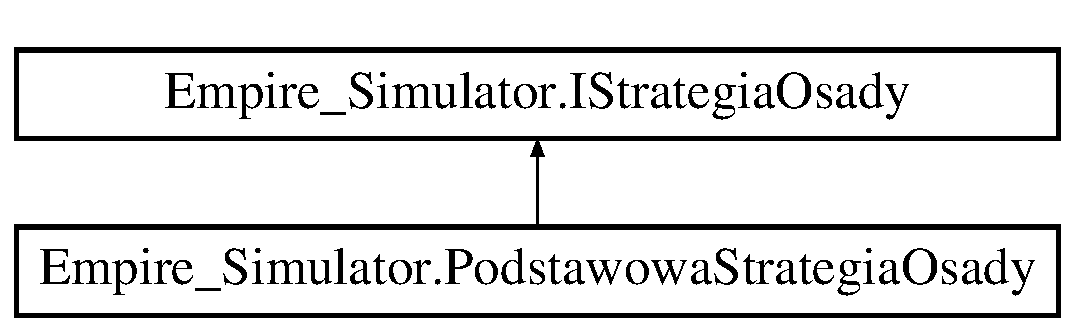
\includegraphics[height=2.000000cm]{class_empire___simulator_1_1_podstawowa_strategia_osady}
\end{center}
\end{figure}
\subsection*{Public Member Functions}
\begin{DoxyCompactItemize}
\item 
void \hyperlink{class_empire___simulator_1_1_podstawowa_strategia_osady_a44cd6153770830086b7616b657d90e4e}{aktualizuj\+Stan\+Populacji} (\hyperlink{class_empire___simulator_1_1_populacja}{Populacja} populacja, \hyperlink{class_empire___simulator_1_1_magazyn}{Magazyn} magazyn)
\begin{DoxyCompactList}\small\item\em Aktualizacja statnu popoulacji polega na zwiekszeniu lub zmiejszeniu populacji w zaleznosci od konkretnej strategi \end{DoxyCompactList}\item 
void \hyperlink{class_empire___simulator_1_1_podstawowa_strategia_osady_acf471696a52414814bd0608005c9518d}{aktualizuj\+Stany\+Magazynowe} (\hyperlink{class_empire___simulator_1_1_magazyn}{Magazyn} magazyn, \hyperlink{class_empire___simulator_1_1_potencjal_wydobywczy}{Potencjal\+Wydobywczy} potencjal\+Wydobywczy, int liczba\+Ludnosci)
\begin{DoxyCompactList}\small\item\em (w takiej prostej strategi przyjmuje ze kazda osoba wykorzystuje 1 kazdego surowca w wiosce, dodatkowo produkujac 2 surowca ktory jest wydobywany w danej wiosce) \end{DoxyCompactList}\end{DoxyCompactItemize}


\subsection{Detailed Description}
Własna strategia implementujaca interfejs strategi osady 



\subsection{Member Function Documentation}
\hypertarget{class_empire___simulator_1_1_podstawowa_strategia_osady_a44cd6153770830086b7616b657d90e4e}{\index{Empire\+\_\+\+Simulator\+::\+Podstawowa\+Strategia\+Osady@{Empire\+\_\+\+Simulator\+::\+Podstawowa\+Strategia\+Osady}!aktualizuj\+Stan\+Populacji@{aktualizuj\+Stan\+Populacji}}
\index{aktualizuj\+Stan\+Populacji@{aktualizuj\+Stan\+Populacji}!Empire\+\_\+\+Simulator\+::\+Podstawowa\+Strategia\+Osady@{Empire\+\_\+\+Simulator\+::\+Podstawowa\+Strategia\+Osady}}
\subsubsection[{aktualizuj\+Stan\+Populacji}]{\setlength{\rightskip}{0pt plus 5cm}void Empire\+\_\+\+Simulator.\+Podstawowa\+Strategia\+Osady.\+aktualizuj\+Stan\+Populacji (
\begin{DoxyParamCaption}
\item[{{\bf Populacja}}]{populacja, }
\item[{{\bf Magazyn}}]{stan\+Magazynowy}
\end{DoxyParamCaption}
)\hspace{0.3cm}{\ttfamily [inline]}}}\label{class_empire___simulator_1_1_podstawowa_strategia_osady_a44cd6153770830086b7616b657d90e4e}


Aktualizacja statnu popoulacji polega na zwiekszeniu lub zmiejszeniu populacji w zaleznosci od konkretnej strategi 


\begin{DoxyParams}{Parameters}
{\em populacja} & \\
\hline
{\em stan\+Magazynowy} & \\
\hline
\end{DoxyParams}


Implements \hyperlink{interface_empire___simulator_1_1_i_strategia_osady_ac9ee9a6f745e76c2869f7561dfce9dd5}{Empire\+\_\+\+Simulator.\+I\+Strategia\+Osady}.

\hypertarget{class_empire___simulator_1_1_podstawowa_strategia_osady_acf471696a52414814bd0608005c9518d}{\index{Empire\+\_\+\+Simulator\+::\+Podstawowa\+Strategia\+Osady@{Empire\+\_\+\+Simulator\+::\+Podstawowa\+Strategia\+Osady}!aktualizuj\+Stany\+Magazynowe@{aktualizuj\+Stany\+Magazynowe}}
\index{aktualizuj\+Stany\+Magazynowe@{aktualizuj\+Stany\+Magazynowe}!Empire\+\_\+\+Simulator\+::\+Podstawowa\+Strategia\+Osady@{Empire\+\_\+\+Simulator\+::\+Podstawowa\+Strategia\+Osady}}
\subsubsection[{aktualizuj\+Stany\+Magazynowe}]{\setlength{\rightskip}{0pt plus 5cm}void Empire\+\_\+\+Simulator.\+Podstawowa\+Strategia\+Osady.\+aktualizuj\+Stany\+Magazynowe (
\begin{DoxyParamCaption}
\item[{{\bf Magazyn}}]{magazyn, }
\item[{{\bf Potencjal\+Wydobywczy}}]{potencjal\+Wydobywczy, }
\item[{int}]{liczba\+Ludnosci}
\end{DoxyParamCaption}
)\hspace{0.3cm}{\ttfamily [inline]}}}\label{class_empire___simulator_1_1_podstawowa_strategia_osady_acf471696a52414814bd0608005c9518d}


(w takiej prostej strategi przyjmuje ze kazda osoba wykorzystuje 1 kazdego surowca w wiosce, dodatkowo produkujac 2 surowca ktory jest wydobywany w danej wiosce) 


\begin{DoxyParams}{Parameters}
{\em magazyn} & \\
\hline
{\em potencjal\+Wydobywczy} & \\
\hline
{\em liczba\+Ludnosci} & \\
\hline
\end{DoxyParams}


Implements \hyperlink{interface_empire___simulator_1_1_i_strategia_osady_a79abecf2ba585fb74915ed89fd7b06d6}{Empire\+\_\+\+Simulator.\+I\+Strategia\+Osady}.



The documentation for this class was generated from the following file\+:\begin{DoxyCompactItemize}
\item 
C\+:/\+Users/\+Paweł/\+Documents/\+Git\+Hub/\+Empire\+\_\+\+Simulator\+\_\+\+V\+S\+\_\+2008/\+Empire\+\_\+\+Simulator/\+Empire\+\_\+\+Simulator/\+Strategie/Podstawowa\+Strategia\+Osady.\+cs\end{DoxyCompactItemize}

\hypertarget{class_empire___simulator_1_1_populacja}{\section{Empire\+\_\+\+Simulator.\+Populacja Class Reference}
\label{class_empire___simulator_1_1_populacja}\index{Empire\+\_\+\+Simulator.\+Populacja@{Empire\+\_\+\+Simulator.\+Populacja}}
}


Klasa Tworzaca obiekty populacji tj zawierajace informacie o liczbie ludnosci  


\subsection*{Public Member Functions}
\begin{DoxyCompactItemize}
\item 
\hypertarget{class_empire___simulator_1_1_populacja_a4287735452b732a6c6d16e594a354097}{{\bfseries Populacja} (int liczba\+Populacji)}\label{class_empire___simulator_1_1_populacja_a4287735452b732a6c6d16e594a354097}

\item 
int \hyperlink{class_empire___simulator_1_1_populacja_aee4754bb3c5c73f8eee553cb5af8cf7e}{liczba\+Ludnosci} ()
\begin{DoxyCompactList}\small\item\em zwraca informacje o liczbie ludnosci \end{DoxyCompactList}\item 
void \hyperlink{class_empire___simulator_1_1_populacja_ae34999adbd8cff5ab9471a1b806374b0}{zmien\+Liczbe\+Ludnosci} (int wartosc)
\begin{DoxyCompactList}\small\item\em metoda do zmiany liczebnosci populacji, na razie jesli nie ma wystarczajacej liczby ludnosci zeby zmniejszyc ustawiamy ja na zero \end{DoxyCompactList}\end{DoxyCompactItemize}


\subsection{Detailed Description}
Klasa Tworzaca obiekty populacji tj zawierajace informacie o liczbie ludnosci 



\subsection{Member Function Documentation}
\hypertarget{class_empire___simulator_1_1_populacja_aee4754bb3c5c73f8eee553cb5af8cf7e}{\index{Empire\+\_\+\+Simulator\+::\+Populacja@{Empire\+\_\+\+Simulator\+::\+Populacja}!liczba\+Ludnosci@{liczba\+Ludnosci}}
\index{liczba\+Ludnosci@{liczba\+Ludnosci}!Empire\+\_\+\+Simulator\+::\+Populacja@{Empire\+\_\+\+Simulator\+::\+Populacja}}
\subsubsection[{liczba\+Ludnosci}]{\setlength{\rightskip}{0pt plus 5cm}int Empire\+\_\+\+Simulator.\+Populacja.\+liczba\+Ludnosci (
\begin{DoxyParamCaption}
{}
\end{DoxyParamCaption}
)\hspace{0.3cm}{\ttfamily [inline]}}}\label{class_empire___simulator_1_1_populacja_aee4754bb3c5c73f8eee553cb5af8cf7e}


zwraca informacje o liczbie ludnosci 

\begin{DoxyReturn}{Returns}
Intowa wartosc oznaczajaca liczbe ludnosci danej poulacji
\end{DoxyReturn}
\hypertarget{class_empire___simulator_1_1_populacja_ae34999adbd8cff5ab9471a1b806374b0}{\index{Empire\+\_\+\+Simulator\+::\+Populacja@{Empire\+\_\+\+Simulator\+::\+Populacja}!zmien\+Liczbe\+Ludnosci@{zmien\+Liczbe\+Ludnosci}}
\index{zmien\+Liczbe\+Ludnosci@{zmien\+Liczbe\+Ludnosci}!Empire\+\_\+\+Simulator\+::\+Populacja@{Empire\+\_\+\+Simulator\+::\+Populacja}}
\subsubsection[{zmien\+Liczbe\+Ludnosci}]{\setlength{\rightskip}{0pt plus 5cm}void Empire\+\_\+\+Simulator.\+Populacja.\+zmien\+Liczbe\+Ludnosci (
\begin{DoxyParamCaption}
\item[{int}]{wartosc}
\end{DoxyParamCaption}
)\hspace{0.3cm}{\ttfamily [inline]}}}\label{class_empire___simulator_1_1_populacja_ae34999adbd8cff5ab9471a1b806374b0}


metoda do zmiany liczebnosci populacji, na razie jesli nie ma wystarczajacej liczby ludnosci zeby zmniejszyc ustawiamy ja na zero 


\begin{DoxyParams}{Parameters}
{\em wartosc} & \\
\hline
\end{DoxyParams}


The documentation for this class was generated from the following file\+:\begin{DoxyCompactItemize}
\item 
C\+:/\+Users/\+Paweł/\+Documents/\+Git\+Hub/\+Empire\+\_\+\+Simulator\+\_\+\+V\+S\+\_\+2008/\+Empire\+\_\+\+Simulator/\+Empire\+\_\+\+Simulator/\+Klasy/\+Osada/Populacja.\+cs\end{DoxyCompactItemize}

\hypertarget{class_empire___simulator_1_1_potencjal_wydobywczy}{\section{Empire\+\_\+\+Simulator.\+Potencjal\+Wydobywczy Class Reference}
\label{class_empire___simulator_1_1_potencjal_wydobywczy}\index{Empire\+\_\+\+Simulator.\+Potencjal\+Wydobywczy@{Empire\+\_\+\+Simulator.\+Potencjal\+Wydobywczy}}
}


Potencjal wydobywczy bedzie gotowym obiektem zawieajacym liste obiektow zasobu jakie generuje dana osada  


\subsection*{Public Member Functions}
\begin{DoxyCompactItemize}
\item 
\hypertarget{class_empire___simulator_1_1_potencjal_wydobywczy_a2db65c9ca35009c3cf62b6fd7b60f9a8}{{\bfseries Potencjal\+Wydobywczy} (List$<$ string $>$ lista)}\label{class_empire___simulator_1_1_potencjal_wydobywczy_a2db65c9ca35009c3cf62b6fd7b60f9a8}

\item 
List$<$ string $>$ \hyperlink{class_empire___simulator_1_1_potencjal_wydobywczy_a8f5c8a2011d8a2c846cf5ec64c8c1f75}{pobierz\+Potencjal} ()
\begin{DoxyCompactList}\small\item\em metoda zwracajaca liste potencjalu \end{DoxyCompactList}\item 
\hypertarget{class_empire___simulator_1_1_potencjal_wydobywczy_ae54d0ffe93497d5d210fc1f635d8d348}{override string {\bfseries To\+String} ()}\label{class_empire___simulator_1_1_potencjal_wydobywczy_ae54d0ffe93497d5d210fc1f635d8d348}

\end{DoxyCompactItemize}


\subsection{Detailed Description}
Potencjal wydobywczy bedzie gotowym obiektem zawieajacym liste obiektow zasobu jakie generuje dana osada 



\subsection{Member Function Documentation}
\hypertarget{class_empire___simulator_1_1_potencjal_wydobywczy_a8f5c8a2011d8a2c846cf5ec64c8c1f75}{\index{Empire\+\_\+\+Simulator\+::\+Potencjal\+Wydobywczy@{Empire\+\_\+\+Simulator\+::\+Potencjal\+Wydobywczy}!pobierz\+Potencjal@{pobierz\+Potencjal}}
\index{pobierz\+Potencjal@{pobierz\+Potencjal}!Empire\+\_\+\+Simulator\+::\+Potencjal\+Wydobywczy@{Empire\+\_\+\+Simulator\+::\+Potencjal\+Wydobywczy}}
\subsubsection[{pobierz\+Potencjal}]{\setlength{\rightskip}{0pt plus 5cm}List$<$string$>$ Empire\+\_\+\+Simulator.\+Potencjal\+Wydobywczy.\+pobierz\+Potencjal (
\begin{DoxyParamCaption}
{}
\end{DoxyParamCaption}
)\hspace{0.3cm}{\ttfamily [inline]}}}\label{class_empire___simulator_1_1_potencjal_wydobywczy_a8f5c8a2011d8a2c846cf5ec64c8c1f75}


metoda zwracajaca liste potencjalu 

\begin{DoxyReturn}{Returns}

\end{DoxyReturn}


The documentation for this class was generated from the following file\+:\begin{DoxyCompactItemize}
\item 
C\+:/\+Users/\+Paweł/\+Documents/\+Git\+Hub/\+Empire\+\_\+\+Simulator\+\_\+\+V\+S\+\_\+2008/\+Empire\+\_\+\+Simulator/\+Empire\+\_\+\+Simulator/\+Klasy/\+Zasob/Potencjal\+Wydobywczy.\+cs\end{DoxyCompactItemize}

\hypertarget{class_empire___simulator_1_1_swiat}{\section{Empire\+\_\+\+Simulator.\+Swiat Class Reference}
\label{class_empire___simulator_1_1_swiat}\index{Empire\+\_\+\+Simulator.\+Swiat@{Empire\+\_\+\+Simulator.\+Swiat}}
}


Obekt klasy swiat jest takim \char`\"{}kontenerem\char`\"{} trzymajcaym liste osad i liste handlarzy dostepnych w aktualnym świecie  


\subsection*{Public Member Functions}
\begin{DoxyCompactItemize}
\item 
\hypertarget{class_empire___simulator_1_1_swiat_a1c15c0646552179b890ff084367739f4}{{\bfseries Swiat} (List$<$ \hyperlink{class_empire___simulator_1_1_osada}{Osada} $>$ lista\+Osad, List$<$ \hyperlink{class_empire___simulator_1_1_handlarz}{Handlarz} $>$ lista\+Handlarzy)}\label{class_empire___simulator_1_1_swiat_a1c15c0646552179b890ff084367739f4}

\item 
\hypertarget{class_empire___simulator_1_1_swiat_ab33f910469e0e57c26c9815a4b388803}{void {\bfseries dodaj\+Osade} (\hyperlink{class_empire___simulator_1_1_osada}{Osada} osada)}\label{class_empire___simulator_1_1_swiat_ab33f910469e0e57c26c9815a4b388803}

\item 
\hypertarget{class_empire___simulator_1_1_swiat_ad8f446dc6f49d9d9486196b3d0976928}{void {\bfseries dodaj\+Handlarza} (\hyperlink{class_empire___simulator_1_1_handlarz}{Handlarz} handlarz)}\label{class_empire___simulator_1_1_swiat_ad8f446dc6f49d9d9486196b3d0976928}

\item 
\hypertarget{class_empire___simulator_1_1_swiat_af29f44d2f029fdd2d88020f637481428}{List$<$ \hyperlink{class_empire___simulator_1_1_handlarz}{Handlarz} $>$ {\bfseries pobierz\+Liste\+Handlarzy} ()}\label{class_empire___simulator_1_1_swiat_af29f44d2f029fdd2d88020f637481428}

\item 
\hypertarget{class_empire___simulator_1_1_swiat_a3309a2122299ea8483639aadd5eb075f}{List$<$ \hyperlink{class_empire___simulator_1_1_osada}{Osada} $>$ {\bfseries pobierz\+Liste\+Osad} ()}\label{class_empire___simulator_1_1_swiat_a3309a2122299ea8483639aadd5eb075f}

\end{DoxyCompactItemize}


\subsection{Detailed Description}
Obekt klasy swiat jest takim \char`\"{}kontenerem\char`\"{} trzymajcaym liste osad i liste handlarzy dostepnych w aktualnym świecie 



The documentation for this class was generated from the following file\+:\begin{DoxyCompactItemize}
\item 
C\+:/\+Users/\+Paweł/\+Documents/\+Git\+Hub/\+Empire\+\_\+\+Simulator\+\_\+\+V\+S\+\_\+2008/\+Empire\+\_\+\+Simulator/\+Empire\+\_\+\+Simulator/\+Klasy/\+Swiat/Swiat.\+cs\end{DoxyCompactItemize}

\hypertarget{class_empire___simulator_1_1_targ}{\section{Empire\+\_\+\+Simulator.\+Targ Class Reference}
\label{class_empire___simulator_1_1_targ}\index{Empire\+\_\+\+Simulator.\+Targ@{Empire\+\_\+\+Simulator.\+Targ}}
}


\hyperlink{class_empire___simulator_1_1_targ}{Targ} posiadany przez miasto i uzywany do komunikacji miedzy handlarzami a miastem  


\subsection*{Public Member Functions}
\begin{DoxyCompactItemize}
\item 
\hypertarget{class_empire___simulator_1_1_targ_a60eb64c3d36cf5483bb68cfb39cee9b4}{{\bfseries Targ} (\hyperlink{class_empire___simulator_1_1_magazyn}{Magazyn} magazyn, \hyperlink{interface_empire___simulator_1_1_i_strategia_handlu}{I\+Strategia\+Handlu} strategia, List$<$ string $>$ co\+Sprzedawac)}\label{class_empire___simulator_1_1_targ_a60eb64c3d36cf5483bb68cfb39cee9b4}

\item 
void \hyperlink{class_empire___simulator_1_1_targ_a88a802730bc74d2f256d97700b98a102}{Wymiana\+Towaru} (\hyperlink{class_empire___simulator_1_1_handlarz}{Handlarz} handlarz)
\begin{DoxyCompactList}\small\item\em wymiany uzywam ze strategi handlu \end{DoxyCompactList}\end{DoxyCompactItemize}


\subsection{Detailed Description}
\hyperlink{class_empire___simulator_1_1_targ}{Targ} posiadany przez miasto i uzywany do komunikacji miedzy handlarzami a miastem 



\subsection{Member Function Documentation}
\hypertarget{class_empire___simulator_1_1_targ_a88a802730bc74d2f256d97700b98a102}{\index{Empire\+\_\+\+Simulator\+::\+Targ@{Empire\+\_\+\+Simulator\+::\+Targ}!Wymiana\+Towaru@{Wymiana\+Towaru}}
\index{Wymiana\+Towaru@{Wymiana\+Towaru}!Empire\+\_\+\+Simulator\+::\+Targ@{Empire\+\_\+\+Simulator\+::\+Targ}}
\subsubsection[{Wymiana\+Towaru}]{\setlength{\rightskip}{0pt plus 5cm}void Empire\+\_\+\+Simulator.\+Targ.\+Wymiana\+Towaru (
\begin{DoxyParamCaption}
\item[{{\bf Handlarz}}]{handlarz}
\end{DoxyParamCaption}
)\hspace{0.3cm}{\ttfamily [inline]}}}\label{class_empire___simulator_1_1_targ_a88a802730bc74d2f256d97700b98a102}


wymiany uzywam ze strategi handlu 


\begin{DoxyParams}{Parameters}
{\em handlarz} & \\
\hline
\end{DoxyParams}


The documentation for this class was generated from the following file\+:\begin{DoxyCompactItemize}
\item 
C\+:/\+Users/\+Paweł/\+Documents/\+Git\+Hub/\+Empire\+\_\+\+Simulator\+\_\+\+V\+S\+\_\+2008/\+Empire\+\_\+\+Simulator/\+Empire\+\_\+\+Simulator/\+Klasy/\+Osada/Targ.\+cs\end{DoxyCompactItemize}

\hypertarget{class_empire___simulator_1_1_test}{\section{Empire\+\_\+\+Simulator.\+Test Class Reference}
\label{class_empire___simulator_1_1_test}\index{Empire\+\_\+\+Simulator.\+Test@{Empire\+\_\+\+Simulator.\+Test}}
}


The documentation for this class was generated from the following file\+:\begin{DoxyCompactItemize}
\item 
C\+:/\+Users/\+Paweł/\+Documents/\+Git\+Hub/\+Empire\+\_\+\+Simulator\+\_\+\+V\+S\+\_\+2008/\+Empire\+\_\+\+Simulator/\+Empire\+\_\+\+Simulator/Test.\+cs\end{DoxyCompactItemize}

\hypertarget{class_empire___simulator_1_1_text_box_label}{\section{Empire\+\_\+\+Simulator.\+Text\+Box\+Label Class Reference}
\label{class_empire___simulator_1_1_text_box_label}\index{Empire\+\_\+\+Simulator.\+Text\+Box\+Label@{Empire\+\_\+\+Simulator.\+Text\+Box\+Label}}
}


Kod skopiowany z iternetu obsługujący przeźroczystość text\+Boxów  


Inheritance diagram for Empire\+\_\+\+Simulator.\+Text\+Box\+Label\+:\begin{figure}[H]
\begin{center}
\leavevmode
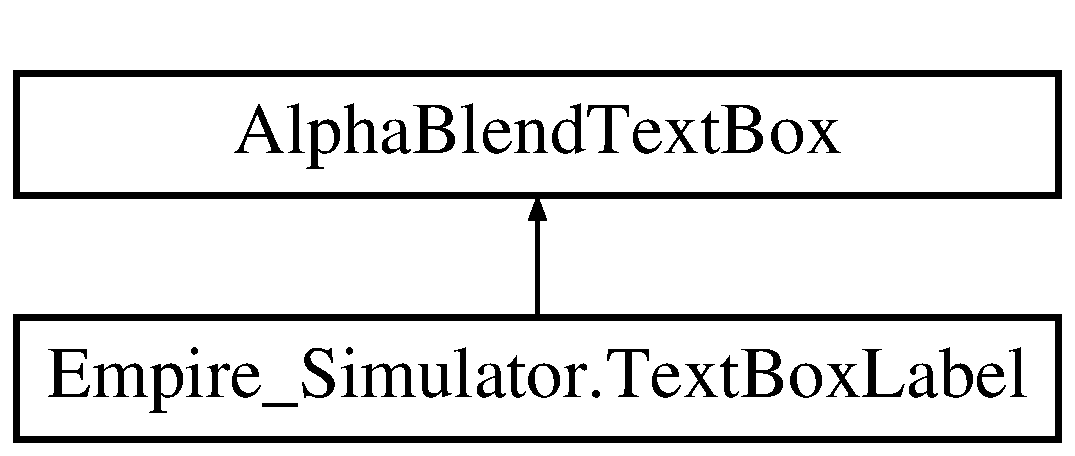
\includegraphics[height=2.000000cm]{class_empire___simulator_1_1_text_box_label}
\end{center}
\end{figure}
\subsection*{Protected Member Functions}
\begin{DoxyCompactItemize}
\item 
\hypertarget{class_empire___simulator_1_1_text_box_label_ab9210551caa97acc31317d77142c6418}{override void {\bfseries Wnd\+Proc} (ref Message m)}\label{class_empire___simulator_1_1_text_box_label_ab9210551caa97acc31317d77142c6418}

\end{DoxyCompactItemize}


\subsection{Detailed Description}
Kod skopiowany z iternetu obsługujący przeźroczystość text\+Boxów 



The documentation for this class was generated from the following file\+:\begin{DoxyCompactItemize}
\item 
C\+:/\+Users/\+Paweł/\+Documents/\+Git\+Hub/\+Empire\+\_\+\+Simulator\+\_\+\+V\+S\+\_\+2008/\+Empire\+\_\+\+Simulator/\+Empire\+\_\+\+Simulator/\+Mapa/Generator\+Mapy.\+cs\end{DoxyCompactItemize}

\hypertarget{class_empire___simulator_1_1_woz_handlarza}{\section{Empire\+\_\+\+Simulator.\+Woz\+Handlarza Class Reference}
\label{class_empire___simulator_1_1_woz_handlarza}\index{Empire\+\_\+\+Simulator.\+Woz\+Handlarza@{Empire\+\_\+\+Simulator.\+Woz\+Handlarza}}
}


klasa woz handlarza bedzie obiektem trzymajacym zasoby przewozone przez Handlarza uzywam slownika dlatego ze w przyszlosci planuje to ze handlarz bedzie wozil kilka roznych towarow  


\subsection*{Public Member Functions}
\begin{DoxyCompactItemize}
\item 
\hypertarget{class_empire___simulator_1_1_woz_handlarza_ae1de7eb5d33e5f74909d25628e759164}{{\bfseries Woz\+Handlarza} (int ladownosc)}\label{class_empire___simulator_1_1_woz_handlarza_ae1de7eb5d33e5f74909d25628e759164}

\item 
void \hyperlink{class_empire___simulator_1_1_woz_handlarza_a9946b05459f36955d26386b8bc91076d}{laduj} (Key\+Value\+Pair$<$ string, \hyperlink{class_empire___simulator_1_1_zasob}{Zasob} $>$ towar)
\begin{DoxyCompactList}\small\item\em laduje towar o konkretnej nazwie i ilosci na woz (przepelnienie do ogarniecia) \end{DoxyCompactList}\item 
Key\+Value\+Pair$<$ string, \hyperlink{class_empire___simulator_1_1_zasob}{Zasob} $>$ \hyperlink{class_empire___simulator_1_1_woz_handlarza_a5dfcb6e147923716145ba925b1b457b8}{rozladuj} ()
\begin{DoxyCompactList}\small\item\em Rozladowuje towar z wozu handlarza zwracajac ilosc surowca oczywiscie narazie żeby tylko działało, wiec bez zadnego sprawdzania. \end{DoxyCompactList}\item 
\hypertarget{class_empire___simulator_1_1_woz_handlarza_a3dbe23380236fb9eaa6851abaf59cd3e}{string {\bfseries Nazwa\+Przewozonego\+Zasobu} ()}\label{class_empire___simulator_1_1_woz_handlarza_a3dbe23380236fb9eaa6851abaf59cd3e}

\item 
\hypertarget{class_empire___simulator_1_1_woz_handlarza_afe055447c6b88b189bbf9e6667809abc}{override string {\bfseries To\+String} ()}\label{class_empire___simulator_1_1_woz_handlarza_afe055447c6b88b189bbf9e6667809abc}

\end{DoxyCompactItemize}


\subsection{Detailed Description}
klasa woz handlarza bedzie obiektem trzymajacym zasoby przewozone przez Handlarza uzywam slownika dlatego ze w przyszlosci planuje to ze handlarz bedzie wozil kilka roznych towarow 



\subsection{Member Function Documentation}
\hypertarget{class_empire___simulator_1_1_woz_handlarza_a9946b05459f36955d26386b8bc91076d}{\index{Empire\+\_\+\+Simulator\+::\+Woz\+Handlarza@{Empire\+\_\+\+Simulator\+::\+Woz\+Handlarza}!laduj@{laduj}}
\index{laduj@{laduj}!Empire\+\_\+\+Simulator\+::\+Woz\+Handlarza@{Empire\+\_\+\+Simulator\+::\+Woz\+Handlarza}}
\subsubsection[{laduj}]{\setlength{\rightskip}{0pt plus 5cm}void Empire\+\_\+\+Simulator.\+Woz\+Handlarza.\+laduj (
\begin{DoxyParamCaption}
\item[{Key\+Value\+Pair$<$ string, {\bf Zasob} $>$}]{towar}
\end{DoxyParamCaption}
)\hspace{0.3cm}{\ttfamily [inline]}}}\label{class_empire___simulator_1_1_woz_handlarza_a9946b05459f36955d26386b8bc91076d}


laduje towar o konkretnej nazwie i ilosci na woz (przepelnienie do ogarniecia) 

\hypertarget{class_empire___simulator_1_1_woz_handlarza_a5dfcb6e147923716145ba925b1b457b8}{\index{Empire\+\_\+\+Simulator\+::\+Woz\+Handlarza@{Empire\+\_\+\+Simulator\+::\+Woz\+Handlarza}!rozladuj@{rozladuj}}
\index{rozladuj@{rozladuj}!Empire\+\_\+\+Simulator\+::\+Woz\+Handlarza@{Empire\+\_\+\+Simulator\+::\+Woz\+Handlarza}}
\subsubsection[{rozladuj}]{\setlength{\rightskip}{0pt plus 5cm}Key\+Value\+Pair$<$string, {\bf Zasob}$>$ Empire\+\_\+\+Simulator.\+Woz\+Handlarza.\+rozladuj (
\begin{DoxyParamCaption}
{}
\end{DoxyParamCaption}
)\hspace{0.3cm}{\ttfamily [inline]}}}\label{class_empire___simulator_1_1_woz_handlarza_a5dfcb6e147923716145ba925b1b457b8}


Rozladowuje towar z wozu handlarza zwracajac ilosc surowca oczywiscie narazie żeby tylko działało, wiec bez zadnego sprawdzania. 

\begin{DoxyReturn}{Returns}
ilosc surowca
\end{DoxyReturn}


The documentation for this class was generated from the following file\+:\begin{DoxyCompactItemize}
\item 
C\+:/\+Users/\+Paweł/\+Documents/\+Git\+Hub/\+Empire\+\_\+\+Simulator\+\_\+\+V\+S\+\_\+2008/\+Empire\+\_\+\+Simulator/\+Empire\+\_\+\+Simulator/\+Klasy/\+Handlarz/Woz\+Handlarza.\+cs\end{DoxyCompactItemize}

\hypertarget{class_empire___simulator_1_1_zasob}{\section{Empire\+\_\+\+Simulator.\+Zasob Class Reference}
\label{class_empire___simulator_1_1_zasob}\index{Empire\+\_\+\+Simulator.\+Zasob@{Empire\+\_\+\+Simulator.\+Zasob}}
}


Obiekt zasobu przechowujacy jego nazwe wage i ilosc  


\subsection*{Public Member Functions}
\begin{DoxyCompactItemize}
\item 
\hypertarget{class_empire___simulator_1_1_zasob_a4003837db3e3421e869e6da2ecf13e8f}{{\bfseries Zasob} (string nazwa, int ilosc, int waga)}\label{class_empire___simulator_1_1_zasob_a4003837db3e3421e869e6da2ecf13e8f}

\item 
string \hyperlink{class_empire___simulator_1_1_zasob_a54ab3a43784f56fcb03062678ca7b191}{nazwa\+Zasobu} ()
\begin{DoxyCompactList}\small\item\em Zwracajaca nazwe zasobu przechowywanego w obiekcie \end{DoxyCompactList}\item 
int \hyperlink{class_empire___simulator_1_1_zasob_aeebc81eccdc0d9117de6d1aedd680711}{ilosc\+Zasobu} ()
\begin{DoxyCompactList}\small\item\em Zwracajaca ilosc zasobu przechowywanego w klasie \end{DoxyCompactList}\item 
void \hyperlink{class_empire___simulator_1_1_zasob_a6736e29b299f7dbb7651934b47fb9694}{zmien\+Ilosc\+Zasobu} (int wartosc)
\begin{DoxyCompactList}\small\item\em Metoda zmieniajaca ilosc zasobu o podana wartosc, ujemna albo dodatnią Na razie przyjalem że gdy nie mam wystarczajcych zasobow na pokrycie czegos wartosc mojego zasobu sie zeruje \end{DoxyCompactList}\item 
\hypertarget{class_empire___simulator_1_1_zasob_a980dc48881144d0e8686135a64eb3277}{int {\bfseries zwroc\+Wage\+Zasobu} ()}\label{class_empire___simulator_1_1_zasob_a980dc48881144d0e8686135a64eb3277}

\item 
\hypertarget{class_empire___simulator_1_1_zasob_aaee5a41fce840c8e6780a758e7e07228}{override string {\bfseries To\+String} ()}\label{class_empire___simulator_1_1_zasob_aaee5a41fce840c8e6780a758e7e07228}

\end{DoxyCompactItemize}


\subsection{Detailed Description}
Obiekt zasobu przechowujacy jego nazwe wage i ilosc 



\subsection{Member Function Documentation}
\hypertarget{class_empire___simulator_1_1_zasob_aeebc81eccdc0d9117de6d1aedd680711}{\index{Empire\+\_\+\+Simulator\+::\+Zasob@{Empire\+\_\+\+Simulator\+::\+Zasob}!ilosc\+Zasobu@{ilosc\+Zasobu}}
\index{ilosc\+Zasobu@{ilosc\+Zasobu}!Empire\+\_\+\+Simulator\+::\+Zasob@{Empire\+\_\+\+Simulator\+::\+Zasob}}
\subsubsection[{ilosc\+Zasobu}]{\setlength{\rightskip}{0pt plus 5cm}int Empire\+\_\+\+Simulator.\+Zasob.\+ilosc\+Zasobu (
\begin{DoxyParamCaption}
{}
\end{DoxyParamCaption}
)\hspace{0.3cm}{\ttfamily [inline]}}}\label{class_empire___simulator_1_1_zasob_aeebc81eccdc0d9117de6d1aedd680711}


Zwracajaca ilosc zasobu przechowywanego w klasie 

\begin{DoxyReturn}{Returns}
intowa ilosc zasobu
\end{DoxyReturn}
\hypertarget{class_empire___simulator_1_1_zasob_a54ab3a43784f56fcb03062678ca7b191}{\index{Empire\+\_\+\+Simulator\+::\+Zasob@{Empire\+\_\+\+Simulator\+::\+Zasob}!nazwa\+Zasobu@{nazwa\+Zasobu}}
\index{nazwa\+Zasobu@{nazwa\+Zasobu}!Empire\+\_\+\+Simulator\+::\+Zasob@{Empire\+\_\+\+Simulator\+::\+Zasob}}
\subsubsection[{nazwa\+Zasobu}]{\setlength{\rightskip}{0pt plus 5cm}string Empire\+\_\+\+Simulator.\+Zasob.\+nazwa\+Zasobu (
\begin{DoxyParamCaption}
{}
\end{DoxyParamCaption}
)\hspace{0.3cm}{\ttfamily [inline]}}}\label{class_empire___simulator_1_1_zasob_a54ab3a43784f56fcb03062678ca7b191}


Zwracajaca nazwe zasobu przechowywanego w obiekcie 

\begin{DoxyReturn}{Returns}
string z nazwa
\end{DoxyReturn}
\hypertarget{class_empire___simulator_1_1_zasob_a6736e29b299f7dbb7651934b47fb9694}{\index{Empire\+\_\+\+Simulator\+::\+Zasob@{Empire\+\_\+\+Simulator\+::\+Zasob}!zmien\+Ilosc\+Zasobu@{zmien\+Ilosc\+Zasobu}}
\index{zmien\+Ilosc\+Zasobu@{zmien\+Ilosc\+Zasobu}!Empire\+\_\+\+Simulator\+::\+Zasob@{Empire\+\_\+\+Simulator\+::\+Zasob}}
\subsubsection[{zmien\+Ilosc\+Zasobu}]{\setlength{\rightskip}{0pt plus 5cm}void Empire\+\_\+\+Simulator.\+Zasob.\+zmien\+Ilosc\+Zasobu (
\begin{DoxyParamCaption}
\item[{int}]{wartosc}
\end{DoxyParamCaption}
)\hspace{0.3cm}{\ttfamily [inline]}}}\label{class_empire___simulator_1_1_zasob_a6736e29b299f7dbb7651934b47fb9694}


Metoda zmieniajaca ilosc zasobu o podana wartosc, ujemna albo dodatnią Na razie przyjalem że gdy nie mam wystarczajcych zasobow na pokrycie czegos wartosc mojego zasobu sie zeruje 


\begin{DoxyParams}{Parameters}
{\em wartosc} & \\
\hline
\end{DoxyParams}


The documentation for this class was generated from the following file\+:\begin{DoxyCompactItemize}
\item 
C\+:/\+Users/\+Paweł/\+Documents/\+Git\+Hub/\+Empire\+\_\+\+Simulator\+\_\+\+V\+S\+\_\+2008/\+Empire\+\_\+\+Simulator/\+Empire\+\_\+\+Simulator/\+Klasy/\+Zasob/Zasob.\+cs\end{DoxyCompactItemize}

%--- End generated contents ---

% Index
\newpage
\phantomsection
\addcontentsline{toc}{chapter}{Index}
\printindex

\end{document}
